% Arquivo LaTeX de exemplo de dissertação/tese a ser apresentada à CPG do IME-USP
%
% Criação: Jesús P. Mena-Chalco
% Revisão: Fabio Kon e Paulo Feofiloff
% Adaptação para UTF8, biblatex e outras melhorias: Nelson Lago
%
% Except where otherwise indicated, these files are distributed under
% the MIT Licence. The example text, which includes the tutorial and
% examples as well as the explanatory comments in the source, are
% available under the Creative Commons Attribution International
% Licence, v4.0 (CC-BY 4.0) - https://creativecommons.org/licenses/by/4.0/


%%%%%%%%%%%%%%%%%%%%%%%%%%%%%%%%%%%%%%%%%%%%%%%%%%%%%%%%%%%%%%%%%%%%%%%%%%%%%%%%
%%%%%%%%%%%%%%%%%%%%%%%%%%%%%%% PREÂMBULO LaTeX %%%%%%%%%%%%%%%%%%%%%%%%%%%%%%%%
%%%%%%%%%%%%%%%%%%%%%%%%%%%%%%%%%%%%%%%%%%%%%%%%%%%%%%%%%%%%%%%%%%%%%%%%%%%%%%%%

% A opção twoside (frente-e-verso) significa que a aparência das páginas pares
% e ímpares pode ser diferente. Por exemplo, as margens podem ser diferentes ou
% os números de página podem aparecer à direita ou à esquerda alternadamente.
% Mas nada impede que você crie um documento "só frente" e, ao imprimir, faça
% a impressão frente-e-verso.
%
% Aqui também definimos a língua padrão do documento (a última da lista) e
% línguas adicionais. Para teses do IME, no mínimo português e inglês são
% obrigatórios, porque independentemente da língua principal do texto é
% preciso fornecer o resumo nessas duas línguas. LaTeX aceita alguns nomes
% diferentes para a língua portuguesa; dentre as opções, prefira sempre
% "brazilian" para português brasileiro e "portuguese" para português europeu.
\documentclass[a4paper,12pt,twoside,brazilian,english]{book}
%\documentclass[a4paper,12pt,twoside,english,brazilian]{book}

% O preâmbulo de um documento LaTeX pode ser razoavelmente longo. Neste
% modelo, optamos por reduzi-lo, colocando praticamente tudo do preâmbulo
% nas packages "imegoodies" e "imelooks".
%
% imegoodies carrega diversas packages muito úteis e populares (algumas
% são praticamente obrigatórias, como amsmath, babel, array etc.). É
% uma boa ideia usá-la com outros documentos também. Ela inclui vários
% comentários explicativos e dicas de uso; não tenha medo de alterá-la
% conforme a necessidade.
%
% imelooks carrega algumas packages e configurações que definem a
% aparência do documento; você também pode querer usá-la (ou partes
% dela) com outros documentos para obter as mesmas fontes, margens
% etc. Tal como "imegoodies", pode valer a pena ler os comentários
% e fazer modificações nessa package. Com a opção "thesis", imelooks
% também define os comandos para capa, folha de rosto etc.
\usepackage{imegoodies}
\usepackage[thesis]{imelooks}

%\nocolorlinks % para impressão em P&B

% Diretórios onde estão as figuras; com isso, não é necessário (mas
% é permitido) colocar o caminho completo em \includegraphics. Note
% que a extensão nunca é necessária (mas é permitida), ou seja, o
% resultado é o mesmo com "\includegraphics{figuras/foto.jpeg}",
% "\includegraphics{foto.jpeg}", "\includegraphics{figuras/foto}"
% ou "\includegraphics{foto}".
\graphicspath{{figuras/},{fig/},{logos/},{img/},{images/},{imagens/}}

% Comandos rápidos para mudar de língua:
% \en -> muda para o inglês
% \br -> muda para o português
% \texten{blah} -> o texto "blah" é em inglês
% \textbr{blah} -> o texto "blah" é em português
\babeltags{br = brazilian, en = english}


%%%%%%%%%%%%%%%%%%%%%%%%%%%%%%%%%%%%%%%%%%%%%%%%%%%%%%%%%%%%%%%%%%%%%%%%%%%%%%%%
%%%%%%%%%%%%%%%%%%%%%%%%%%%%%%%%%% METADADOS %%%%%%%%%%%%%%%%%%%%%%%%%%%%%%%%%%%
%%%%%%%%%%%%%%%%%%%%%%%%%%%%%%%%%%%%%%%%%%%%%%%%%%%%%%%%%%%%%%%%%%%%%%%%%%%%%%%%

% O arquivo com os dados bibliográficos para biblatex; você pode usar
% este comando mais de uma vez para acrescentar múltiplos arquivos
\addbibresource{bibliografia.bib}

% Este comando permite acrescentar itens à lista de referências sem incluir
% uma referência de fato no texto (pode ser usado em qualquer lugar do texto)
%\nocite{bronevetsky02,schmidt03:MSc, FSF:GNU-GPL, CORBA:spec, MenaChalco08}
% Com este comando, todos os itens do arquivo .bib são incluídos na lista
% de referências
%\nocite{*}

% É possível definir como determinadas palavras podem (ou não) ser
% hifenizadas; no entanto, a hifenização automática geralmente funciona bem
\babelhyphenation{documentclass latexmk soft-ware clsguide} % todas as línguas
\babelhyphenation[brazilian]{Fu-la-no}
\babelhyphenation[english]{what-ever}

% Estes comandos definem o título e autoria do trabalho e devem sempre ser
% definidos, pois além de serem utilizados para criar a capa, também são
% armazenados nos metadados do PDF. O subtítulo é opcional.
\title{An approach for detecting and mitigating code duplication in the Linux Kernel}
\translatedtitle{Uma abordagem para detecção e mitigação de código duplicado no Linux Kernel}

\author[fem]{Luan Ícaro Pinto Arcanjo}

\def\profa{Prof\kern.02em.\kern-.07emª\kern.07em}
\def\dra{Dr\kern-.04em.\kern-.11emª\kern.07em}

% Para TCCs, este comando define o supervisor
\orientador{\profa{} \dra{} Paulo Meirelles}

\banca{
  \profa{} \dra{} Fulana de Tal (orientadora) -- IME-USP [sem ponto final],
  % Em inglês, não há o "ª"
  %Prof. Dr. Fulana de Tal (advisor) -- IME-USP [sem ponto final],
  Prof. Dr. Ciclano de Tal -- IME-USP [sem ponto final],
  \profa{} \dra{} Convidada de Tal -- IMPA [sem ponto final],
}

% A página de rosto da versão para depósito (ou seja, a versão final
% antes da defesa) deve ser diferente da página de rosto da versão
% definitiva (ou seja, a versão final após a incorporação das sugestões
% da banca).
\tipotese{
  mestrado,
  %doutorado,
  %tcc,
  %definitiva, % É a versão para defesa ou a versão definitiva?
  quali, % É qualificação?
  programa={Ciência da Computação},
}

\defesa{
  local={São Paulo},
  data=2024-01-01, % YYYY-MM-DD
}

% Se não houve bolsa, remova
%
% Norma sobre agradecimento por auxílios da FAPESP:
% https://fapesp.br/11789/referencia-ao-apoio-da-fapesp-em-todas-as-formas-de-divulgacao
%
% Norma sobre agradecimento por auxílios da CAPES (Portaria 206,
% de 4 de Setembro de 2018):
% https://www.in.gov.br/materia/-/asset_publisher/Kujrw0TZC2Mb/content/id/39729251/do1-2018-09-05-portaria-n-206-de-4-de-setembro-de-2018-39729135
%
%\apoio{O presente trabalho foi realizado com apoio da Coordenação
%      de Aperfeiçoamento\\ de Pessoal de Nível Superior -- Brasil
%      (CAPES) -- Código de Financiamento 001} % o código é sempre 001
%
%\apoio{This study was financed in part by the Coordenação de
%      Aperfeiçoamento\\ de Pessoal de Nível Superior -- Brasil
%      (CAPES) -- Finance Code 001} % o código é sempre 001
%
%\apoio{Durante o desenvolvimento deste trabalho, o autor recebeu\\
%      auxílio financeiro da FAPESP -- processo nº aaaa/nnnnn-d}
%
%\apoio{During the development if this work, the author received\\
%      financial support from FAPESP -- grant \#aaaa/nnnnn-d}
%\apoio{Durante o desenvolvimento deste trabalho o autor
%       recebeu auxílio financeiro da XXXX}

% A licença do seu trabalho. Use CC-BY, CC-BY-NC, CC-BY-ND, CC-BY-SA,
% CC-BY-NC-SA ou CC-BY-NC-ND para escolher a licença Creative Commons
% correspondente (o sistema insere automaticamente o texto da licença).
% Se quiser estabelecer regras diferentes para o uso de seu trabalho,
% converse com seu orientador e coloque o texto da licença aqui, mas
% observe que apenas TCCs sob alguma licença Creative Commons serão
% acrescentados ao BDTA. Se você tem alguma intenção de publicar o
% trabalho comercialmente no futuro, sugerimos a licença CC-BY-NC-ND.
%
%\direitos{CC-BY-NC-ND}
%
%\direitos{Autorizo a reprodução e divulgação total ou parcial deste
%          trabalho, por qualquer meio convencional ou eletrônico,
%          para fins de estudo e pesquisa, desde que citada a fonte.}
%
%\direitos{I authorize the complete or partial reproduction and disclosure
%          of this work by any conventional or electronic means for study
%          and research purposes, provided that the source is acknowledged.}
%
\direitos{CC-BY}

% Para gerar a ficha catalográfica, acesse https://fc.ime.usp.br/,
% preencha o formulário e escolha a opção "Gerar Código LaTeX".
% Basta copiar e colar o resultado aqui.
\fichacatalografica{}


%%%%%%%%%%%%%%%%%%%%%%%%%%%%%%%%%%%%%%%%%%%%%%%%%%%%%%%%%%%%%%%%%%%%%%%%%%%%%%%%
%%%%%%%%%%%%%%%%%%%%%%% AQUI COMEÇA O CONTEÚDO DE FATO %%%%%%%%%%%%%%%%%%%%%%%%%
%%%%%%%%%%%%%%%%%%%%%%%%%%%%%%%%%%%%%%%%%%%%%%%%%%%%%%%%%%%%%%%%%%%%%%%%%%%%%%%%

\begin{document}

%%%%%%%%%%%%%%%%%%%%%%%%%%% CAPA E PÁGINAS INICIAIS %%%%%%%%%%%%%%%%%%%%%%%%%%%%

% Aqui começa o conteúdo inicial que aparece antes do capítulo 1, ou seja,
% página de rosto, resumo, sumário etc. O comando frontmatter faz números
% de página aparecem em algarismos romanos ao invés de arábicos e
% desabilita a contagem de capítulos.
\frontmatter

\pagestyle{plain}

\onehalfspacing % Espaçamento 1,5 na capa e páginas iniciais

\maketitle % capa e folha de rosto

%%%%%%%%%%%%%%%% DEDICATÓRIA, AGRADECIMENTOS, RESUMO/ABSTRACT %%%%%%%%%%%%%%%%%%

%\begin{dedicatoria}
%Esta seção é opcional e fica numa página separada; ela pode ser usada para
%uma dedicatória ou epígrafe.
%\end{dedicatoria}

% Reinicia o contador de páginas (a próxima página recebe o número "i") para
% que a página da dedicatória não seja contada.
\pagenumbering{roman}

% Agradecimentos:
% Se o candidato não quer fazer agradecimentos, deve simplesmente eliminar
% esta página. A epígrafe, obviamente, é opcional; é possível colocar
% epígrafes em todos os capítulos. O comando "\chapter*" faz esta seção
% não ser incluída no sumário.
% \chapter*{Agradecimentos}
% \epigrafe{Do. Or do not. There is no try.}{Mestre Yoda}
% 
% Texto texto texto texto texto texto texto texto texto texto texto texto texto
% texto texto texto texto texto texto texto texto texto texto texto texto texto
% texto texto texto texto texto texto texto texto texto texto texto texto texto
% texto texto texto texto. Texto opcional.

%!TeX root=../tese.tex
%("dica" para o editor de texto: este arquivo é parte de um documento maior)
% para saber mais: https://tex.stackexchange.com/q/78101

% As palavras-chave são obrigatórias, em português e em inglês, e devem ser
% definidas antes do resumo/abstract. Acrescente quantas forem necessárias.
\palavraschave{Software livre, kernel Linux, duplicação de código, refatoração, manutenção de software}

\keywords{Free software,Linux kernel, Code duplication, Refactoring, code maintenance}

% O resumo é obrigatório, em português e inglês. Estes comandos também
% geram automaticamente a referência para o próprio documento, conforme
% as normas sugeridas da USP.
\resumo{

O kernel Linux é um projeto de software livre amplamente utilizado, alimentando 96,3\% 
dos um milhão maiores servidores web e 85\% dos smartphones em todo o mundo. Dada a sua extensa 
base de usuários, qualquer adição de recursos, correção de bugs ou tratamento de 
vulnerabilidades de segurança pode impactar milhões de pessoas. Manter o kernel é 
uma tarefa enorme, envolvendo mais de 19 milhões de linhas de código e contribuições 
de mais de mil desenvolvedores. Devido à escala do projeto, nem todas as contribuições 
seguem as melhores práticas, resultando em artefatos de código de baixa qualidade que 
podem complicar a manutenção e o desenvolvimento de novos recursos. Um desses artefatos 
é a duplicação de código, que é o foco desta pesquisa. As ferramentas existentes 
para detectar duplicação de código normalmente comparam dois artefatos de código para 
determinar se são duplicatas. No entanto, essas ferramentas não são adequadas para 
identificar duplicações em bases de código em grande escala, como o kernel Linux, nem 
oferecem orientações sobre como resolver as duplicações detectadas. Apesar das 
pesquisas tanto na literatura formal quanto na cinza, as soluções existentes não 
conseguem resolver os desafios específicos do kernel Linux. 
Esta pesquisa apresenta o ArKanjo, uma ferramenta de linha de comando para a manutenção 
do kernel Linux, projetada para detectar e analisar duplicações em nível de função. 
Lançado sob a licença MIT, o ArKanjo emprega uma arquitetura de dois estágios que consiste 
em um Preprocessor e um Query Responder, que separa a análise computacionalmente intensiva 
da consulta eficiente por duplicações em grandes bases de código. Em segundo lugar, ele 
analisa as duplicações identificadas para extrair padrões e métodos de refatoração, oferecendo 
orientação a futuros contribuidores. Avaliamos o ArKanjo em casos de duplicação do mundo 
real em versões recentes do kernel, demonstrando sua eficácia na identificação de clones 
problemáticos que ferramentas genéricas frequentemente ignoram. Ao identificar instâncias 
de duplicação bem definidas e gerenciáveis, o ArKanjo reduz efetivamente a barreira para 
novos contribuidores, uma capacidade evidenciada por seu papel em orientar estudantes a 
fazerem suas primeiras melhorias de código no kernel.

}

\abstract{

The Linux kernel is a widely used Free/Libre/Open Source Software (FLOSS) project, powering
96.3\% of the top one million web servers 
and 85\% of smartphones worldwide. Given its extensive user base, any addition of features, 
bug fixes, or handling of security vulnerabilities can impact millions. Maintaining the kernel 
is an enormous task involving over 28 million lines of code and contributions from over 
twenty thousand developers. Due to the scale of the project, not all contributions adhere to best 
practices, resulting in poor-quality code artifacts that may complicate maintenance and feature 
development. One such artifact is code duplication, which is the focus of this research. 
Existing tools for detecting code duplication typically compare two code artifacts to determine 
if they are duplicates. However, these tools are not well-suited for identifying duplications 
in large-scale codebases like the Linux kernel, nor do they guide on resolving detected 
duplications. Despite searches in both formal and grey literature, existing solutions fall 
short of addressing the specific challenges of the Linux kernel.
This research presents ArKanjo  , a command-line tool for Linux kernel maintenance designed to detect and
analyze function-level duplications. Released under the MIT
license, ArKanjo employs a two-stage architecture consisting
of a Preprocessor and a Query Responder that separates
computationally intensive analysis from efficient querying for duplications within large codebases.
Second, it analyzes the identified duplications to extract patterns 
and refactoring methods, offering guidance to future contributors. We evaluate ArKanjo 
against real-world duplication cases in recent kernel versions, demonstrating
its effectiveness in identifying problematic clones that generic
tools often overlook. By identifying well-defined, manageable
duplication instances, ArKanjo effectively lowers the barrier
for new contributors, a capability evidenced by its role in guiding students to make their first 
code improvements to the kernel.

}



%%%%%%%%%%%%%%%%%%%%%%%%%%% LISTAS DE FIGURAS ETC. %%%%%%%%%%%%%%%%%%%%%%%%%%%%%

% Como as listas que se seguem podem não incluir uma quebra de página
% obrigatória, inserimos uma quebra manualmente aqui.
\cleardoublepage

% Todas as listas são opcionais; Usando "\chapter*" elas não são incluídas
% no sumário. As listas geradas automaticamente também não são incluídas por
% conta das opções "notlot" e "notlof" que usamos para a package tocbibind.

% Normalmente, "\chapter*" faz o novo capítulo iniciar em uma nova página, e as
% listas geradas automaticamente também por padrão ficam em páginas separadas.
% Como cada uma destas listas é muito curta, não faz muito sentido fazer isso
% aqui, então usamos este comando para desabilitar essas quebras de página.
% Se você preferir, comente as linhas com esse comando e des-comente as linhas
% sem ele para criar as listas em páginas separadas. Observe que você também
% pode inserir quebras de página manualmente (com \clearpage, veja o exemplo
% mais abaixo).
\newcommand\disablenewpage[1]{{\let\clearpage\par\let\cleardoublepage\par #1}}

% Nestas listas, é melhor usar "raggedbottom" (veja basics.tex). Colocamos
% a opção correspondente e as listas dentro de um grupo para ativar
% raggedbottom apenas temporariamente.
\bgroup
\raggedbottom

%%%%% Listas criadas manualmente

%\chapter*{Lista de abreviaturas}
\disablenewpage{\chapter*{List of abbreviations}}

\begin{tabular}{rl}
   T1 & Type-1 of Code Clone Duplication\\
   T2 & Type-2 of Code Clone Duplication\\
   T3 & Type-3 of Code Clone Duplication\\
   T4 & Type-4 of Code Clone Duplication\\
   ST3 & Strong Type-3 of Code Clone Duplication\\
   MT3 & Medium Type-3 of Code Clone Duplication\\
   WT3 & Weak Type-3 of Code Clone Duplication\\
   GNU & GNU’s Not Unix! \\
   IME & Instituto de Matemática e Estatística\\
   USP & Universidade de São Paulo
\end{tabular}

%\chapter*{Lista de símbolos}
%\disablenewpage{\chapter*{Lista de símbolos}}
%
%\begin{tabular}{rl}
%  $\omega$ & Frequência angular\\
%    $\psi$ & Função de análise \emph{wavelet}\\
%    $\Psi$ & Transformada de Fourier de $\psi$\\
%\end{tabular}

% Quebra de página manual
\clearpage

%%%%% Listas criadas automaticamente

% Você pode escolher se quer ou não permitir a quebra de página
%\listoffigures
\disablenewpage{\listoffigures}

% Você pode escolher se quer ou não permitir a quebra de página
%\listoftables
\disablenewpage{\listoftables}

% Esta lista é criada "automaticamente" pela package float quando
% definimos o novo tipo de float "program" (em utils.tex)
% Você pode escolher se quer ou não permitir a quebra de página
%\listof{program}{\programlistname}
%\disablenewpage{\listof{program}{\programlistname}}

% Sumário (obrigatório)
\tableofcontents

\egroup % Final de "raggedbottom"

% Referências indiretas ("x", veja "y") para o índice remissivo (opcionais,
% pois o índice é opcional). É comum colocar esses itens no final do documento,
% junto com o comando \printindex, mas em alguns casos isso torna necessário
% executar texindy (ou makeindex) mais de uma vez, então colocar aqui é melhor.
\index{Inglês|see{Língua estrangeira}}
\index{Figuras|see{Floats}}
\index{Tabelas|see{Floats}}
\index{Código-fonte|see{Floats}}
\index{Subcaptions|see{Subfiguras}}
\index{Sublegendas|see{Subfiguras}}
\index{Equações|see{Modo matemático}}
\index{Fórmulas|see{Modo matemático}}
\index{Rodapé, notas|see{Notas de rodapé}}
\index{Captions|see{Legendas}}
\index{Versão original|see{Tese/Dissertação, versões}}
\index{Versão corrigida|see{Tese/Dissertação, versões}}
\index{Palavras estrangeiras|see{Língua estrangeira}}
\index{Floats!Algoritmo|see{Floats, ordem}}


%%%%%%%%%%%%%%%%%%%%%%%%%%%%%%%% CAPÍTULOS %%%%%%%%%%%%%%%%%%%%%%%%%%%%%%%%%%%%%

% Aqui vai o conteúdo principal do trabalho, ou seja, os capítulos que compõem
% a dissertação/tese. O comando mainmatter reinicia a contagem de páginas,
% modifica a numeração para números arábicos e ativa a contagem de capítulos.
\mainmatter

\pagestyle{mainmatter}

% Espaçamento simples
\singlespacing

% A introdução não tem número de capítulo, então os cabeçalhos também não
\pagestyle{unnumberedchapter}
%!TeX root=../tese.tex
%("dica" para o editor de texto: este arquivo é parte de um documento maior)
% para saber mais: https://tex.stackexchange.com/q/78101

%% ------------------------------------------------------------------------- %%

% "\chapter" cria um capítulo com número e o coloca no sumário; "\chapter*"
% cria um capítulo sem número e não o coloca no sumário. A introdução não
% deve ser numerada, mas deve aparecer no sumário. Por conta disso, este
% modelo define o comando "\chapter**".
\chapter**{Introduction}
\label{cap:introduction}

\en

The Linux kernel is a widely used Free/Libre/Open Source Software (FLOSS) project, 
powering 96.3\% of the top one million web servers and 85\% of smartphones worldwide. 
Maintaining the kernel is an enormous task, involving more than 28 million lines of 
code and contributions from over twenty thousand developers
\footnote{Data directly extracted from Linux github repository \citep{linuxrepo}.
Counted  28783390 lines of code and 20699 number of contributors in May 29th, 2025.
Number of contributors counted as number of unique full name listed as author of a patch.}.
Due to the scale of the project, not all contributions adhere to best practices, resulting 
in poor-quality code artifacts that may complicate maintenance and future feature development.

One such artifact is code duplication, which is the focus of this research. The motivation for 
this work began with a practical problem rooted in device drivers, which are a major part 
of the kernel, representing 66\% of the source code\citep{marcelo}. We interacted with the 
maintainers of the AMD Display driver, an essential component for the 19\% of personal GPUs 
manufactured by AMD in 2023\citep{gpumarket}. They shared their challenges with a significant 
amount of duplicated code that hampers the driver's maintenance. In searching for a solution, 
we found that existing tools are not well-suited for identifying duplications in large-scale 
codebases like the Linux kernel, nor do they offer guidance on how to resolve the duplications 
they find. Despite searching both formal and grey literature, existing solutions fell short of 
addressing these specific challenges. The list of related tools examined in this exploratory 
research is available in Appendix \ref{app:gray}.

This research presents ArKanjo, a command-line tool designed to detect and analyze function-level 
duplications in the Linux kernel. Released under the MIT license, ArKanjo uses a two-stage 
architecture with a Preprocessor and a Query Responder. This design separates the heavy 
computational analysis from the fast querying of duplication results, making it effective for 
large codebases. We validated the tool by comparing its results with the BigCloneBench dataset
\citep{bigclonebench} and by conducting an empirical analysis on a randomly selected set of 
files from the AMD Display driver.

Beyond detection, we also investigated if the duplications found by ArKanjo could be mitigated.
This was achieved through an ethnographic approach, which included a participant observation 
study where we attempted to mitigate duplications, and a non-participant observation study of 
university students tasked with fixing duplications found by the tool. These studies showed that 
ArKanjo can effectively lower the barrier for new contributors, as evidenced by its role in 
guiding students to make their first code contributions to the kernel.

\section**{Research Design}

\label{sec:intresearch}

To address the code duplication problem within the Linux kernel, this research employs a 
multi-method approach designed to bridge the gap between detection and practical mitigation. 
Our approach, illustrated in Figure \ref{fig:reDesign}, is structured into two interconnected phases that progress 
from tool development to an in-depth study of its application within the kernel’s development community. 
The overall objective is to produce not only a functional tool but also actionable insights into 
the patterns and practices surrounding code duplication and its resolution.

\begin{figure}[h]
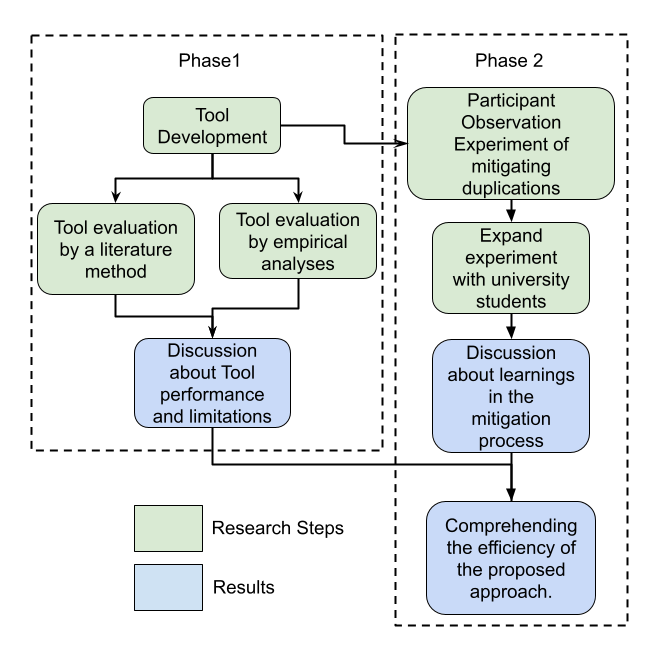
\includegraphics[scale=0.9]{research_design}
\caption{Diagram of the research design.}
\label{fig:reDesign}
\end{figure}

The initial phase of our research focused on the development and validation of ArKanjo, a 
command-line tool capable of identifying code duplication at the function level.  The 
tool's accuracy was rigorously validated by evaluating its performance against the 
standard BigCloneBench dataset \citep{bigclonebench} and by conducting an empirical analysis 
of its results within the AMD Display driver.  This foundational work ensured we had a 
reliable instrument to proceed with the practical investigation of code duplication 
in our target subsystems.

With a validated tool, the research then moved from detection to practice, investigating 
the real-world challenges of mitigating the identified duplications. This was accomplished 
through an ethnographic study designed to engage with the kernel community and understand 
their perspectives on code quality and refactoring.  This study had two components: a 
participant-observation experiment where the author submitted refactoring patches to the 
AMD Display driver, and a non-participant observation of university students using ArKanjo 
to contribute fixes to both the AMD Display and Industrial I/O subsystems.  

By combining tool 
development with direct community interaction, this research design allows for a comprehensive 
understanding of the technical and social factors that influence the mitigation of duplicated 
code in a large-scale open-source project.

\section**{Thesis Structure}

This manuscript consists of five more chapters. Chapter \ref{cha:back} presents
the literature overview for code duplication detection (main definitions,
current approaches in the literature), a brief description of the Linux kernel and the components
explored in this work, 
and a review of refactoring methods used throughout this research. Chapter
\ref{cha:tool} presents ArKanjo, our proposed tool to detect code duplication, 
describing all the main components.  Chapter \ref{cha:method}
describes the research methods selected to guide our work. Chapter
\ref{cha:results} shows the results we had through our work, from the research methods to 
evaluate our tool and the ethnographic studies. Chapter \ref{cha:conclusion} concludes this research.


\pagestyle{mainmatter}
%!TeX root=../tese.tex
%("dica" para o editor de texto: este arquivo é parte de um documento maior)
% para saber mais: https://tex.stackexchange.com/q/78101

\en

\chapter{Background}
\label{cha:back}

\en

This chapter presents an overview of fundamental topics needed to understand 
the research, such as the Linux Kernel, refactoring, types of code duplication, 
code duplication detection methods presented in the literature and ways to 
evaluate these methods. This foundation will make it easier to grasp the 
concepts discussed in the research.

\section{The Linux Kernel}

The Linux kernel, a Unix-like operating system kernel, was published by Linus
Torvalds in 1992 as free software. It began gaining popularity in the late
1990s \citep{linuxbook}. Contrary to popular belief, Linux itself is not a
complete operating system, as it lacks components like filesystem utilities and
windowing systems. The so-called ``Linux distributions'' that are commonly
recognized by the public are actually GNU/Linux operating systems, which
include various essential applications alongside the Linux kernel,
such as system
\citep{gnuref}. Examples of Linux distributions are Ubuntu \citep{ubuntu} 
and Arch Linux \citep{archlinux}.

The Linux kernel is monolithic and organized into subsystems, such as
the process scheduler, memory management, device driver infrastructure,
networking, and filesystems \citep{melissa}. Each subsystem typically has a
dedicated maintainer or a team of maintainers responsible for overseeing its
development and managing contributions \citep{melissa}.

Development contributions to the Linux kernel are coordinated using the Git
version control system. These contributions are formatted as patches—text
documents that outline the differences between two source code versions.
These patches are then submitted and reviewed via the Linux mailing lists
\citep{melissa}.

Mailing lists are the primary means of communication within the Linux
community. Members of the community use them to submit and review patches,
discuss Linux-related topics, and debate potential new features. Given the
kernel's extensive modularity, each subsystem has its mailing list, allowing
discussions to be organized around specific areas of development
\citep{melissa}. All interactions on these mailing lists are documented and
archived in the Linux Kernel Lore \citep{linuxlore}, which serves as a
repository for kernel discussions and can be accessed by anyone interested.

One of the subsystems within the Linux kernel is the AMD Display driver, which
is responsible for implementing the drivers needed for AMD GPUs to function
correctly in a Linux environment. The maintainers of this subsystem have
reported a practical issue: a significant amount of duplicated code, which
complicates the maintenance of this subsystem. This problem serves as the
starting point for our research, with the AMD Display driver as our primary
object of study as we aim to understand and mitigate code duplication in the
Linux kernel. The AMD Display driver subsystem contains more then 391000 lines 
of code and more then 1089 code files
\footnote{ 
Data extracted directly from the Linux repository with the help of the cloc tool.
\citep{cloc}
}, 
making it a considerable component within the Linux kernel. Like other 
subsystems, discussions about the AMD Display driver are conducted on its 
designated mailing list, which can be accessed here: 
\url{https://lists.freedesktop.org/mailman/listinfo/amd-gfx}.

Another subsystem within the Linux kernel explored in this work is the
Industrial I/O subsystem (IIO). According to the Linux kernel documentation, 
''The main purpose of the Industrial I/O subsystem (IIO) is to provide support 
for devices that in some sense perform either analog-to-digital conversion (ADC) 
or digital-to-analog conversion (DAC) or both''\citep{iiodoc}. The IIO subsystem 
contains more than X lines of code and more than Y code files
\footnote{
Data extracted directly from the Linux repository with the help of the clol tool. \citep{cloc}
}.
We opted to include the IIO subsystem in our experiments to ensure our findings 
are not limited to one subsystem. Additionally, we have an established point of
contact within the IIO subsystem to facilitate this work.
Like other subsystems, discussions about the IIO subsytem are conducted on its 
designated mailing list, which can be found here: 
\url{https://subspace.kernel.org/vger.kernel.org.html}.


\subsection{Diff command}

The \textit{diff} command is a command line in Linux that allows the user to compare 
two files line by line \citep{diffcommand}. There are multiple forms in which the command 
results can be shown to the user, and Figure \ref{fig:diff} shows one of them. 
With the command results, it is easy to visualize and extract the number of lines that 
are equal and different between the two compared files.

\begin{figure}
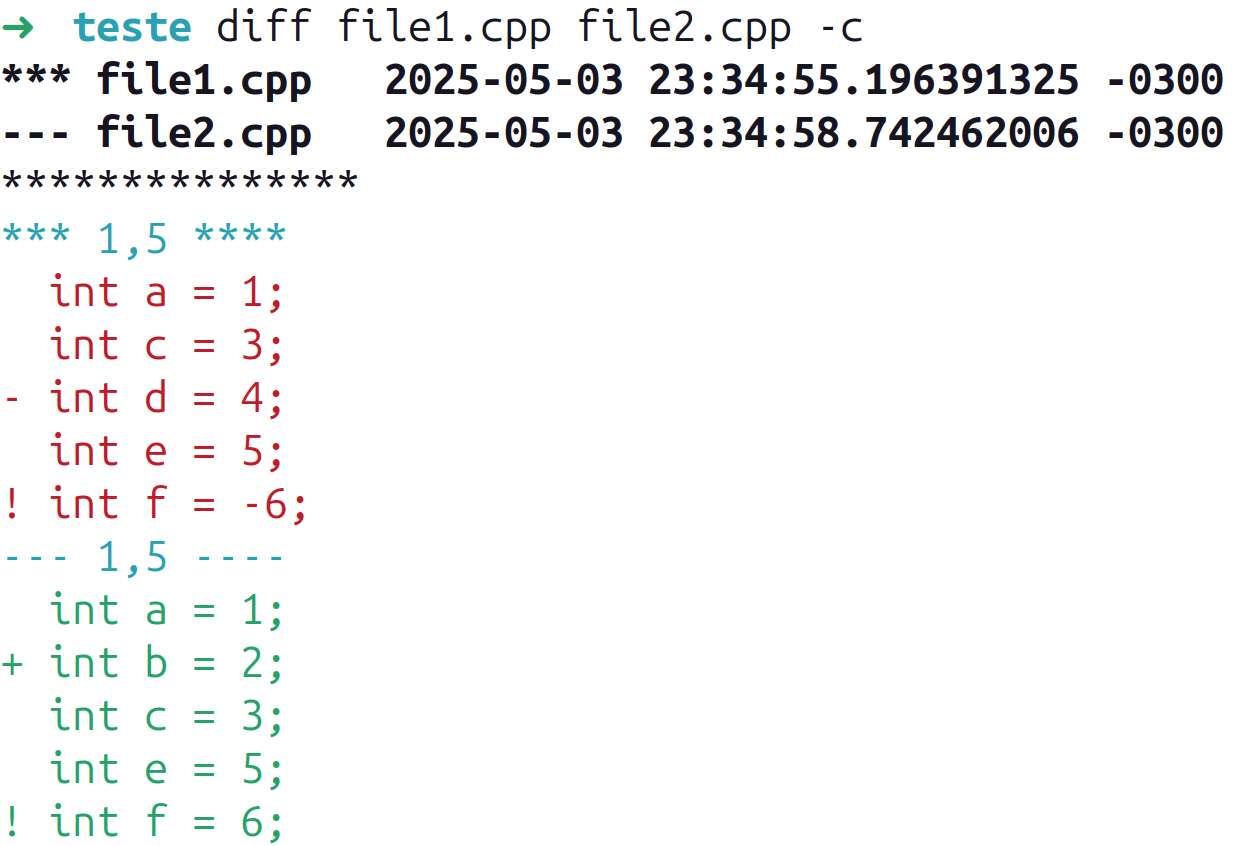
\includegraphics[scale=0.25]{diff_command}
\caption{Example of \textit{diff} command executed}
File 1's content is shown in red, and file 2's content is shown in green. \textit{-} 
represents a line that only exists in file 1, \textit{+} represents a line that only 
exists in file 2,\textit{!} represents a line that exists in both files but has modifications 
between them, and empty at the start of a line represents that the line exists in 
both files without any modifications.
\label{fig:diff}
\end{figure}

We use the \textit{diff} command as the base of one of the code duplication detection 
methods on the tool proposed in this work, although it is not explored as the text 
similarity method for code duplication detection.

\par
\en

\section{Code Duplication Detection}

Code Duplication Detection is a field in computer science studies that gets the attention of researchers 
back to 1988 \citep{firstman}.
The occurrence of Code Duplication is a harmful artifact to have in a software, affecting software related 
tasks such as code readability,
introdution of bugs, etc.   \citep{harmone}. 
On most of the cases, the occurrence of code duplication tends to create a more unstable software then the 
nonduplicate code counterpart.   \citep{harmtwo}

Through the years, the subject of studies about Code Duplication Detection branched out mainly in two fields of study,
Code Clone Detection and Code Plagiarism Detection,
with the former one focused on the technical aspect while the later one also introduces an social aspect on the field of research
\citep{litreview}. For our research we are only interested on the Code Clone Detection branch given the nature of our work.

\subsection{Types of code clone duplication}

\label{subsec:types}

The categorization of two code artifacts as a duplication of each other is a subjective task (REFERENCE HERE). 
To mitigate this human aspect on the given problem, the literature classified code duplication on the scale of changes between 
the code artifacts in four main types of code clone duplication \citep{litreview}. Given two code artifacts F and G, 
the types of Code Duplication are described as follow \citep{litreview}:

\begin{itemize}
	\begin{item}
		\textbf{Type-1:} The differences between F and G are in the context of revision of comments, variable names, white spaces 
		and any other kind of irrelevant elements. (ADD FIGURE) shows a typical example of Type-1 Code 
		Duplication \citep{litreview}. 
	\end{item}
	\begin{item}
		\textbf{Type-2:} The differences between F and G is the same as the type-1, with the addition of considering 
		addition and deletion of redudant codes. (ADD FIGURE) shows a typical example of Type-2 Code Duplication \citep{litreview}. 
	\end{item}
	\begin{item}
		\textbf{Type-3:} The difference between F and G is the same as the type-2, with the addition of considering 
		the reorder of code blocks as well as statements within code blocks. (ADD FIGURE) shows a typical example of 
		Type-3 Code Duplication \citep{litreview}. 
	\end{item}
	\begin{item}
		\textbf{Type-4:} The difference between F and G is the same as the type-3, with the addition of considering 
		changes on data sctrucure, the order of operands/operators in expresssions, or replacing part of codes with 
		equivalent composition. (ADD FIGURE) shows a typical example of Type-4 Code Duplication \citep{litreview}. 
	\end{item}



\end{itemize}

\subsection{Literature approches for code clone detection}

Given the passage of time, the literature developed many techniques and methods to approach the code clone detection problem. 
For better understanding and analyze of these approachs, the literature divided the researches done in
five main methodologies given the main nature of their work \citep{litreview} , which are:

\begin{itemize}
	\item \textbf{Textual-based approaches:} The literature review made by Chen \citep{litreview}  states that this methodology
	is the first to be investigated by the literature. This line of methodology is based on see code as a text artifact and apply
	textual approachs for text similarity. One example of this methodology applied is the work of Roy and Cordy \citep{textexample}, 
	which uses parsing and grammar techniques to detect code clones.

	\item \textbf{Token-based approaches:} This methodoly tries to approach the problem by seeing the code in a similar way to
	the lexical analysis of the compiling process \citep{litreview} . That means doing work in the line of recognizing constants, keywords and other 
	specific programming languages tokens, mapping variables to <pair,value> representations to become naming-independent, etc. One example of 
	this methodology applied  is the work of Toomey et al. \citep{tokenexample} to detect code clones through hashed token sequences.

	\item \textbf{Tree-based approaches:} While the token-based approach uses the lexical analysis of the compiling process, the 
	tree-based approach uses the syntax tree, the structure that  stores the semantic information of a code artifact in respect of the 
	programming language \citep{compiler}. One example of research that uses this information to detect code clones is the one done by
	Chilowicz and Duris \citep{treeexample}.

	\item \textbf{Metric-based approaches:} This methodology approches the problem by extracting metrics from the code artifact and use 
	those metrics as a embedding representation of the artifact to measure similarity \citep{litreview}, similarly to the famous  
	Word2Vec work done by Mikolov et al \citep{wordtovec}. Examples of metrics can be program size, number of variables, number of 
	access to memory, etc. One example of this methodology applied is the work done by Kaur and Sharma. \citep{metricexample}

	\item \textbf{Graph-based approaches:} Similarly to the Tree-based approaches, this methotodology depends heavily on an intermediate
	program representation, called program dependence graph (PDG) \citep{prodg}. The representation store information 
	about program's control, statement and data dependencies. One example of usage of the program dependence graph is 
	the recently work done by Liu et al. \citep{tailor}.
\end{itemize}

The state-of-art methods for code clone detection usually have high computational time and memory space usage, as well being
programming language specific approches, which cannot be easily implemented in programming languagues that were not used in 
their research \citep{litreview}. These are main concern for our research and for this reason we will use a generalist textual-based 
approach based solely on Natural Languague Processing (NLP) text similarity detection methods, which we will introduce and compare
with the literature approches later on this document. 

\subsection{Methodology to evaluate code duplication methods}

\label{subsec:codemethods}

Given the necessity to evaluate and compare approches for code clone detection, it was developed and widely-adopted two datasets: 
OJ-Clone, a dataset collected from a pedagogical online judge system \citep{ojclone}, and BigCloneBench, a dataset collected from over 
25,000 Java software systems \citep{bigclonebench}. The existence of only two spreaded datasets is a open concern in literature as 
the limited scope of OJ-Clone and the problems of BigCloneBench presented by Krinke and Ragkhitwetsagul \citep{bigfail}

(ADD INFORMATION ABOUT THE MORE SEPARATION OF CLONE TYPES THE BIGCLONEBENCH makes)












\par
\en

\section{Text Similarity Detection Methods}
\label{sec:similarity}

The standard methodology for text similarity detection is based on building
vector embeddings of texts and applying a distance function to these embeddings
to measure their similarity. The literature proposes multiple vector
embedding methods, such as bag-of-words, TF-IDF, LSI, and
Word2Vec~\citep{gensimlivro}. Recent works related to vector embedding construction
utilize Large Language Models (LLMs), as exemplified by Ethayarajh's work,
which employs BERT, ELMo, and GPT~\citep{llmsimilar}. The most popular distance
function used in the literature is cosine similarity, defined by the formula~\citep{cosineref}:

$$\text{cosine similarity} = SC(A,B) = \frac{ A \cdot B}{ \lVert A \rVert \lVert B \rVert }$$

Where $A$ and $B$ are the vector embeddings of the two texts. An advantage of
cosine similarity is that $SC(A,B)$ produces a number between $0$ and $1$,
where values closer to $1$ indicate higher similarity. It is common to
interpret cosine similarity as an approximation of probability, transforming
values between $0$ and $1$ into percentages between $0\%$ and $100\%$.
Throughout our research, we will use this percentage form.

It is well-known that LLMs have a high computational cost. For instance, an
analysis by Reimers and Gurevych found that finding the most similar pair in a
collection of 10,000 sentences required about 65 hours with
BERT~\citep{bertsimilar}. Since we aim to compare pairs of similar magnitude in
our work, we decided not to use LLMs for our vector embedding method, even
though they may be suitable for smaller codebases.

\subsection{Gensim}

Gensim is a FLOSS Python library~\citep{gensim}, which its creators
describe as ``The fastest library for training of vector embeddings -- Python or
otherwise. The core algorithms in Gensim use battle-hardened, highly optimized,
and parallelized C routines''~\citep{gensimsite}. Due to Gensim speed, we
chose this library for our vector embedding method.

In this work, we do not explore further alternatives for vector embeddings, as
optimizing computational cost or achieving state-of-the-art code clone
detection is not the primary objective of our research.

\par
\en

\section{Refactoring}

Fowler defines refactoring in his book as "a controlled technique for imporving the design of an existing code base. Its
essence is applying a series of small behavior-preserving transformations, each of which too small to be worth doing. However
the cumulative effect of each of these transformations is quite significant." \citep{refactorbook}. The elimination of detected 
code clone duplication is a refactoring task that necessitates the application of refactoring methods. 
Fowler presents multiples refactoring methods such as parameterize method, replace parameter with explicit methods and 
replace parameter with method \citep{refactorbook}. There is a briefly explanation of the methods used in our research below.

\subsection{Parameterize method}

TODO. I EXPECT TO FILL THIS SECTION AS THE WORK EVOLVES.

\par
\chapter{Proposed tool}
\label{cha:tool}

\en

Arkanjo, our proposed tool, is a Command Line Interface (CLI) application designed to
help developers identify code clone duplication at the function level.
Specifically, it enables the detection of pairs of functions within a codebase
that are clones of each other.

The tool operates in two main parts, the \textbf{Preprocessor} and the \textbf{Query Responder}. 
The \textbf{Preprocessor} is responsible to perform the heavy computations to find the code duplications 
accross a codebase and produce artifact to consulte information related to the duplications in a structured form.
The \textbf{Query Responder} consumes the artifacts produced by the Preprocessor to execute the tool functionalites as requested.
This choice enable the tool to concentrate the heavy and slows parts that can be execute only once per codebase, 
thus allowing a fast performance for multiple queries related to a single codebase.
More detailed descriptions of the Preprocessor and Query Responder can be found in
Sections \ref{subsec:architecture} and \ref{subsec:func}.

The Arkanjo tool has been implemented and is available for reference at
\url{https://github.com/LipArcanjo/arkanjo}.

\todo[inline]{Big maybes: Describe more how the functionalites are implemented, as the focus shifted for the tool as of now.}

\par
\en

\section{Tool architecture}
\label{subsec:architecture}

The Preprocessor contains two main components, the Function Breaker and the Code Duplication Finder. 
The flow of how the Preprocessor works is as follows: Function Parser receives the codebase the user is interested in,
extracts the functions of the codebase along with metadata, and creates a new temporary codebase where the functions extracted become new code files. 
The Code Duplication Finder iterates over every pair of files in the Temporary Codebase, checks if they are code clones, and, 
if so, saves them in the Code Duplication Database, which is a text file that stores every code duplication as a triple 
\textbf{<function1,function2,similarity>}, where \textbf{function1} and \textbf{function2} are the functions that are duplicates 
of each other, and \textbf{similarity} is the metric given by the code duplication detection method utilized in the Code Duplication Finder.

The Query Responder consumes the Temporary Codebase and the Code Duplication Database to extract duplicated 
functions-related information per user request. If the user executes the Query Responder without executing the 
Preprocessor, the Query Responder calls the Preprocessor to create the required artifacts.

Figure~\ref{fig:diagram} illustrates the tool architecture. An explanation of how each component works is provided in this section.

\begin{figure}
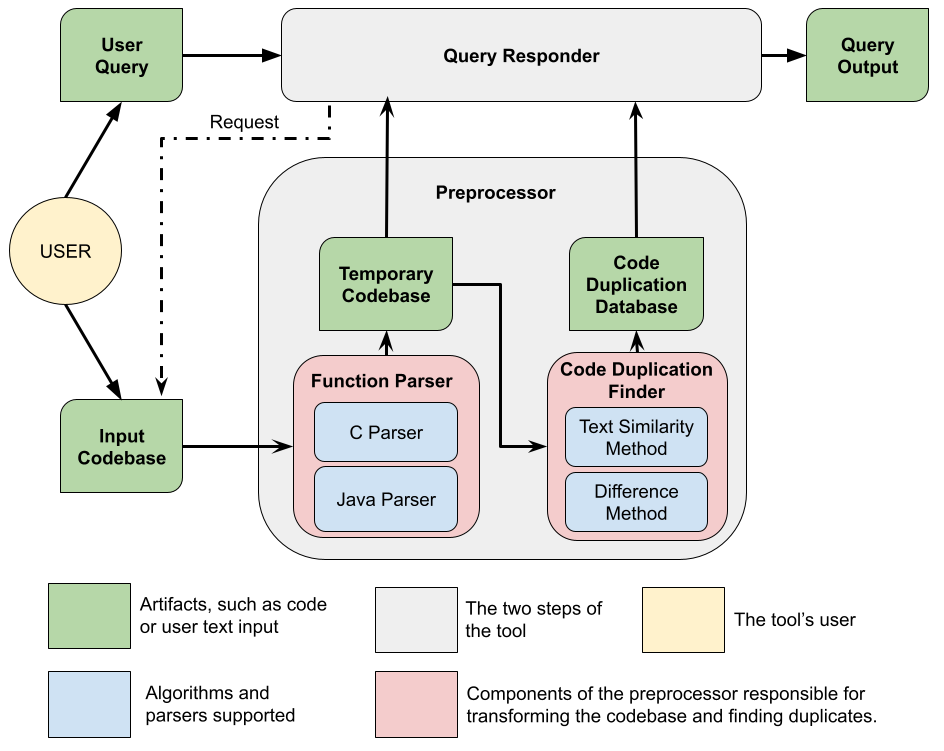
\includegraphics[scale=0.4]{diagrama_mestrado}
\caption{Architecture diagram demonstrating the relationship between the tool components.}
\label{fig:diagram}
\end{figure}

\subsection{Input codebase}

The input codebase is a folder on the machine running the tool. All files in the codebase that are not source code files from a programming language supported by the tool are ignored. The tool validates support for a source file by analyzing its file extension.

\subsection{Function Parser}

The Function Parser receives the input codebase and transforms it into the temporary
codebase. It iterates through every source code file written in a supported programming 
language and uses a language-specific extractor to isolate each function. For each extracted 
function, two new source code files and a metadata file are created in the temporary codebase, 
represented by the pair \textbf{$<$file name, function name$>$}, the source code of the function, 
and the function metadata (in practice, this is a duplication of the original codebase, 
structured as a parsed representation). One of the new files contains the function body, and the other 
contains the function signature. The metadata file includes additional relevant information,
such as the function name, the line where the signature starts, and the line where the function 
body ends. Currently, the supported programming languages are C and Java, although Java support is limited.

\begin{figure}
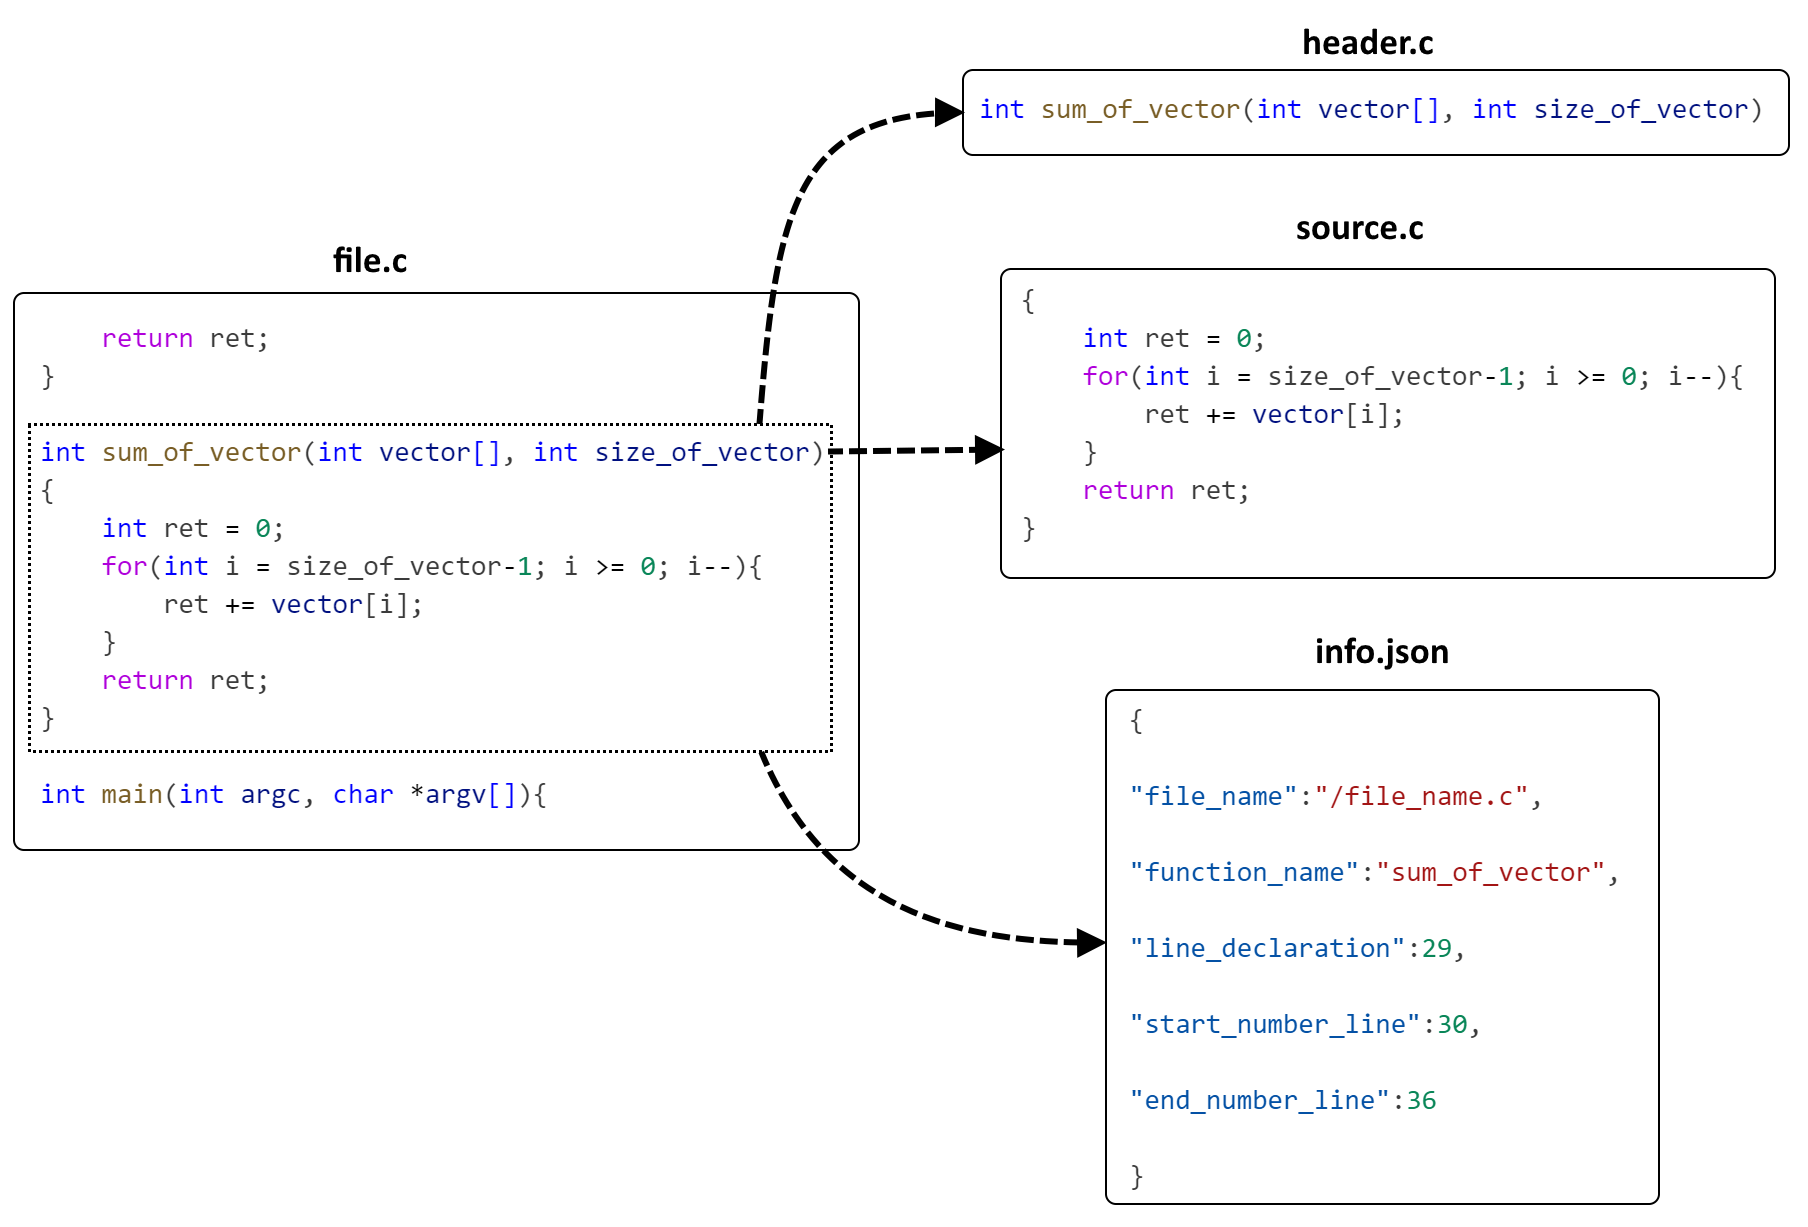
\includegraphics[scale=0.3]{example_function_parser/example_parser}
\caption{Transformation of a function into the temporary codebase}
\label{fig:transform}
\end{figure}

Regarding the programming language function extractor, we approached this problem so that anyone 
comfortable with a language can adapt our approach to their specific programming language. 
Usually, code blocks can be easily extracted from source code files, independently of whether the 
code blocks are defined by curly brackets or by indentation, and it is possible to infer if 
they represent a function body given their depth in the code context and a few lines before the 
start of the code block. We followed this approach to implement the function extractor for the 
supported languages. As an alternative approach, we can build the syntax tree~\citep{compiler} 
of the programming language and use it to extract the functions, which is a more complex task than 
our approach. For the programming languages that we support, we implemented them as follows:

\subsubsection{C Programming Language}

For a source file in the C programming language, we extract the code blocks with depth 0. 
As per the programming language grammar, functions are defined in a global context at depth 0. 
To extract the code blocks, we first need to identify the portions of code that are comments or 
\textit{\#define} directives and mark them as irrelevant. After that, it is simple work to find 
the curly brackets in depth 0; with that, we find the body of the functions.

To extract the header of the functions, we start at the open curly brackets and go back in the 
source file, considering the programming language grammar and the portions of code 
marked as irrelevant because of comments and \textit{\#define} directives.
Other elements in depth zero are not functions; we analyze whether the code blocks 
are functions at the same time that we extract the header of the code block.

\subsubsection{Java Programming Language}

For the Java programming language, we have decided to implement a more straightforward approach 
that does not support the programming language completely, as the only Java codebase explored in 
this work is the BigCloneBench~\citep{bigclonebench}, and the approach implemented covers the 
needs of this codebase.

We extract the code blocks with depth one and some code lines for a source file in Java before 
defining them. Then, we check if the code blocks are functions by analyzing whether the first 
non-empty character before the curly brackets of the code block is a closing parenthesis.

As per Java grammar, functions are defined inside classes and can exist at different depths. 
As Java accepts inner classes, this approach does not work with inner classes. The challenge 
to implementing a more generic approach is that other elements of depth two or deeper, such 
as for-loops, can follow the closing parenthesis pattern, necessitating a better analysis of 
these elements. The BigCloneBench~\citep{bigclonebench} does not contain inner classes.

\subsection{Temporary codebase}

The temporary codebase is a transformation of the input codebase performed by the Function Parser. Each function in the input codebase is represented in the temporary codebase as three files. Descriptions of these files are provided below, with examples shown in Figure~\ref{fig:transform}.

\begin{itemize}
	\item \textbf{Header file}: This file contains the signature of the function it represents.
	\item \textbf{Source file}: This file contains the body of the function it represents.
	\item \textbf{Info file}: This file contains metadata about the function, including the function name, the file that contains the function, the file relative path to the input codebase, the line where the function signature starts, the line where the function body begins, the line where the function body ends, and whether there is a line break between the end of the function signature and the start of the function body.
\end{itemize}

\subsection{Code Duplication Finder}
\label{subsec:code_finder}

The Code Duplication Finder iterates through every pair of source code files in the temporary codebase, representing functions from the input codebase. For each pair of files, we execute a code duplication detection method that computes a metric measuring how similar the pair of files is, which we refer to as similarity. 
If the similarity is greater than or equal to the minimum similarity threshold 
(a parameter provided by the user during the Preprocessor). We store this pair of functions and its 
similarity in the Code Duplication Database.

We implemented two methods for code duplication detection in the tool, which the user can 
use. The first method is based on text similarity, and the second is simpler and 
based on the number of equal lines. The experiments and tests in this research were done 
using the text similarity method. The purpose of the second method is to demonstrate that 
the tool can have multiple duplication detection methods.

\subsubsection{Text Similarity Method}

For the text similarity method, we treat the source code files 
as text and apply the TF-IDF vector embedding method implemented by the 
Gensim library~\citep{gensim}, then compute cosine similarity as the 
similarity metric.

We chose this method for its claimed performance, 
programming language independence, and the fact that it does not require 
compilable code, which is expected in the temporary codebase, as it does 
not contain complete code artifacts. We expect our method to yield good 
results for Type-1 and Type-2 code duplication types while performing 
poorly for others. Changing the code duplication
detection method to one of the state-of-the-art methods is possible if needed.

\cite{platistool} implemented this code duplication detection method and 
released it under the MIT license. We adapted his 
implementation to fit our tool expected input and output formats. 
Switching the duplication detection method is feasible, similar to how 
we adapted Plates' implementation.

\subsubsection{Difference Method}

For the difference method, 
we implemented a method that considered the number of exactly equal lines between two functions.
For two functions \textit{function1} and \textit{function2}, let $NL_1$ be the number of lines in \textit{function1},
$NL_2$ be the number of lines in \textit{function2}, and $EQ$ be the number of equal lines between \textit{function1} and
\textit{function2}, we compute the similarity with the formula:

$$\frac{2 \cdot EQ}{NL_1 + NL_2}$$

This code duplication method is considerably simpler and more explainable than the text similarity method, 
as the metric is the ratio of common lines between the two functions. 
We use the \textit{diff} command built-in the Linux environment \citep{diffcommand}
to compute the number of equal lines.

We did not test the Diff method during the tool evaluation and other phases of this research. 
We implemented the technique to show that a tool can have multiple duplication detection methods.

\subsection{Code Duplication Database}

The Code Duplication Database is a text file that contains the duplicated pairs of functions found by the Code Duplication Finder. The first line of the file specifies the number of duplicated pairs. Following this, each line lists a duplicated pair, including the paths of the functions in the temporary codebase and the similarity metric of the pair.

\subsection{Preprocessor}
\label{subsec:setup}

The Preprocessor is a procedure executed by the user once per codebase. 
The Preprocessor takes the input codebase and a minimum similarity metric value for function pairs considered duplicates. 
It then runs the Function Parser and the Code Duplication Finder to create a temporary codebase and the Code Duplication Database. 
Setting a minimum similarity metric reduces the Code Duplication Database size, optimizing memory usage and the computational 
cost of the Query Responder step. For example, if this parameter does not exist and we work with a codebase of $10,000$ functions, 
each with a 50-character relative path and function name, the Code Duplication Database would reach approximately $5,000^2 \times 50 ~= 5$ gigabytes. 
As most function pairs are unlikely to be duplicated in large codebases, this file size can be significantly reduced.

\subsection{Query Responder}

The Query Responder step is the component that the user executes multiple times to consult information 
about duplicated functions in a codebase processed by the Preprocessor. 
It utilizes the Temporary Codebase and the Code Duplication Database as inputs to answer user requests, 
such as querying for duplicated functions above a certain similarity threshold or providing counts of such functions.
This component was developed to be extensible, allowing other query functionalities to be easily added. 
The specific functionalities provided to the user by the Query Responder, which include the 
Duplication Explorer, Function Information, and Duplication Report, are described in Section~\ref{subsec:func}.


\par
\en

\section{Tool functionalites}
\label{subsec:func}

We proposes three main functionalities for the user in the tool, which are named duplication explorer, function information
and duplication relatory. Each of the functionalities recevies their adequated parameters to execute, with a exception
of a optional parameter shared by all of them, which is minimum similarity per query. The minimum similarity per query is different
from the siminum similarity presented in \ref{subsec:setup}, as it enables a volatile change in the minimum similarity
interested in a query specific context. There is a explanation of each of the main functionalities throughout this section.

\subsection{Duplication explorer}

The duplication explorer is the principal functionality of our tool, the functionality purpose is to expose for the user the code duplication
pairs found by our tool. We implement optional filters methods to enable more complex queries, which are described below. A example
of the functionality usage can be found in (ADD FIGURE HERE).


\begin{itemize}
	\begin{item}
		\textbf{Sorting filter:} This filter enables the user to sort the resuls by similarity of the functions pairs or 
		by the number of duplicated lines. By default the tool sorts by similarity and the user can pass a sort parameter to change
		the sorting method.
	\end{item}

	\begin{item}
		\textbf{Limiter filter:} This filter receives a number parameter named limiter by the user, which limits the number of results
		showed to the user by this given number.
	\end{item}

	\begin{item}
		\textbf{Pattern Filter:} This filter make the explorer ignore every pair of duplicated functions that does not match a pattern
		given by the user as a parameter. We say that a function matches a pattern if the string formed by the concatenation of
		the relative path of the code file plus the function name. The user can define if both functions or at least one of the 
		functions in the pair need to match the pattern by given a specific parameter.
	\end{item}
\end{itemize}


\subsection{Function information}

The Function information purpose it to give a more in depth information about a specific function. The functionality inform the user
about the relative path, the function name and the lines the function exist in the code file that the function is contained for the
function that the user is interested and every function that is a duplication of it. As there ca nbe multiple functions with the 
same name in a codebase, we distinguish then by the user providing a pattern string and we use the first function find that match
the pattern. We say that a function matches a pattern if the string formed by the concatenation of the relative path of the 
code file plus the function name. 
A example of the functionality usage can be found in (ADD FIGURE HERE).

\subsection{Duplication relatory}

The duplication relatory purpose is to give a overview of the input codebase. The functionality extract the information
of how much lines of duplicated code is found per folder in the codebase and present it to the user in a reasonable format. To extract
the information, we use the Code Duplication Database to list the code duplications, and the temporary code to know how much lines of
duplicated code contains in each of the functions. (DO I TALK ABOUT THE TRIE USAGE TO MAINTAIN THE HIERARCHICAL TREE STRUCTURE? I 
THINK NOT). A example of the functionality usage can be found in (ADD FIGURE HERE).






\par

\chapter{Research Methods}
\label{cha:method}

We employ a multi-method research approach, using different methodologies to achieve our goals
to approach code duplication in some of the Linux subsystems. 
To validate if the Arkanjo tool is capable of finding code duplications, 
applied two independent methods and perform triangulation on the results. 

The first method evaluates the proposed tool using an approach from the literature, 
comparing it against the BigCloneBench dataset \citep{bigclonebench}. 
The second method is an empirical analysis of a subset of functions within the 
AMD Display driver that our tool identified as duplicates. After completing these two 
methods, we triangulated the findings to analyze the results comprehensively. 
We chose triangulation because relying solely on the literature-based method has 
limitations and may not be entirely reliable \citep{bigfail, litreview}. As a reminder, 
all research approches were done using the text similarity method as the 
code dupication method of the tool.

Given the validation of the tool's capabilities, we proceed to undertand the viability 
to mitigate the code duplication finds by the tool. 
To underdand the viability, our first choice is to conduct an ethnographic study using 
a participant-observation methodology. 
In this study, we aim to mitigate a subset of duplicated functions by refactoring them 
while interacting with the Linux community to gather feedback on our mitigation efforts. 

The ethnographic study happened in two phases. 
In the first phase, the author of this research explored the process of mitigating
a code duplication found in the AMD Display Driver and sent it as a PATCH to iteract with the
Linux community and get their feedback. On a second phase, we proposed to students on the 
course Free Software Development at University São Paulo to mitigate the code duplications found 
by the tool in the IIO and AMD Display Driver and pass the process of send the mitigations as PATCH.
(DOUBLE CHECK IF THE STUDENTS HAVE SENT THE PATCHES). 

I 

\todo[inline]{The focus of the above section should be a little more on the tool, the introduction about mitigating duplications is good enough. A little about the fact that we will test on IIO later maybe is good. }

\todo[inline]{I SHOULD mention that the test on the tool were made using the gensim similarity method and not the git method.}

\section{Evaluation of the Tool by the BigCloneBench dataset}

\label{sec:metbig}

The BigCloneBench dataset \citep{bigclonebench} is a Java code collection containing pairs of code duplications categorized by clone type, as defined in Section \ref{subsec:types}.
%
Following the methodology presented by \citep{tailor}, we sampled 20,000 pairs from each clone type, adding 20,000 non-duplicate pairs as negative samples. We applied the same sampling approach to our tool to ensure a fair evaluation.

Unlike traditional methods, our tool does not distinguish between clone types and identifies duplications at the function level rather than the file level, which is typical in state-of-the-art tools. Therefore, we adapted the metric calculation method for evaluation purposes. Specifically, we considered every pair of functions with a similarity metric equal to or greater than a threshold \(X\) as duplicates and marked the corresponding file pairs. A correctly identified duplication pair counts as accurate for its clone type, while an incorrectly inferred pair is considered incorrect across all clone types. With these definitions, we computed the Recall metric from Section \ref{subsec:codemethods} for each clone type.
%
To understand the impact of varying the similarity threshold, we evaluated our tool using different threshold values: 30\%, 40\%, 50\%, 60\%, 70\%, 80\%, 90\%, and 100\%. We then analyzed and discussed the results.

\section{Evaluation of the Tool by Empirical Analysis}

\label{sec:metemp}

\todo[inline]{I just mention the problem, maybe a more explictly mention of the problem here or on the background would be good.}

Due to the limitations of the BigCloneBench dataset, as noted by \cite{bigfail}, and its lack of suitability 
for our context (Java dataset vs. C-based Linux kernel), we complemented the BigCloneBench evaluation with 
an empirical study of the tool inferred duplications.

%
Given the vast number of lines and components in the Linux kernel, analyzing every duplication is impractical. We focused our scope on the AMD Display driver, which, as shown in Figure \ref{fig:relatory_ex}, contains over 20,000 lines of duplicated code at a similarity metric of 100\%.

In this empirical analysis, we randomly sampled function pairs identified by the tool as duplicates. For each similarity threshold \(X\) (30\%, 40\%, 50\%, 60\%, 70\%, 80\%, 90\%, and 100\%), we randomly selected ten function pairs with a similarity close to \(X\), allowing for a 1\% deviation. We implemented the random selection using the tool's source code.

Appendix \ref{app:emp} lists the randomly selected function pairs. We empirically evaluated these pairs to determine if they were duplications, comparing these results with the literature-based method to assess our tool's effectiveness and understand the impact of the minimum similarity parameter.

\todo[inline]{Take care: Big focus on AMD display driver and the tone of the writing supports the focus. }

\section{Ethnographic Study}

\label{sec:meteth}

Ethnography is a recognized qualitative empirical method for understanding people, 
their cultures, and their work practices \citep{bookethno}. It allows researchers 
to gain insights into values, beliefs, and ideas from the perspective of community 
members \citep{ethnosoft}. In our research, refactoring code duplications without 
community interaction would prevent us from understanding whether Linux maintainers 
would accept our approach or identify their concerns. Thus, we will use ethnography, 
positioning ourselves as Linux kernel contributors focused on removing identified 
code duplications.

This section outlines our approach for mitigatin code duplication in the Linux kernel
and describes the ethnographic methodology for engagin with the Linux community. Firstly, 
we present the participant observation research method explored by the author. Then, 
we present the methodolody of the experiment done with the students.

\subsection{Participant observation method}


\subsection{Research with students}

\todo[inline]{Rsearch with students does not look good.}

In the Free Software Development course at University of São Paulo, ministred by the advisor 
of this work at the first semester of 2025, we have proposed to the students the possibility
of mitigating duplications in the IIO subsystem and the AMD display driver found with the Arkanjo tool.
The course had a total of X students, and of that, X students being undergraduate students
and Y begin graduate students.

On the course, the students are asked to form groups of one, two or three students and together 
make a contribution to a open source software. To auxiliate the students on this task, the 
professor and teaching assistants prepares multiple alternatives on how to contribute to open source projects, 
including simple contributions as updating documentation or code style fixes. In this context, 
we have proposed two alternatives for the students related to the tool.

For the first alternative, one of the teaching assistants used the Arkanjo tool in the IIO subsystem and
listed interesting duplications that the groups can approach, and it is up to the students on how
to refactor the code to mitigate the duplications and pass through the process to send patches to the IIO 
maintainers to review. For the second alternative, we propose a similar experience then the 
participant observation method, where the students pass through the whole process of executing the Arkanjo tool
in the AMD display driver, analyze the duplications found, create a patch to mitigate a duplication and sent
the patch to the AMD display driver's maintainers.

From the students enrolled in the in the course, X opted for the first alternative and 1 opted for the second
alternative, forming Y groups working on the first alternative and 1 group working on the second alternative. 
These number represent X\% of the students choosing for approching duplications them the other contribution 
alternatives, including more simpler and easy to be done.  It is worth highlighting that none of the students
that choose to mitigate duplications had made a contribution to the Linux kernel before,
meaning that the patch to mitigate the duplication being the first tentative to contribute to the kernel as
newcomers.

The groups have been request to document the experience and approaches to refactor the duplications and the
experience of submiting a patch to the Linux kernel in blogs. We had analyzed these blogs to undertand 
patterns of refactor used for mitigating the duplications, the experience on send the patches and the 
opinions of the subsystem maintainers on the mitigations. Appendix X list the blogs and patches made by the 
student.

For the teaching assistant and the student that has executed the Arkanjo tool to explore duplications, 
we have asked them to answer some questions related to the experience of using the tool and what could be
improved. The question asked can be found below and the answers can be found in Appendix Y.



\par

\chapter{Preliminar Results}
\label{cha:results}

\en 

\todo[inline]{Juntei os capítulos; veja se consegue colocar algo aqui no início; não sei se final remarks é o melhor nome para a segunda secao aqui}

To finalize this report, we present the current state of our research. As of the 
time of writing, we have finished \textbf{Phase I} of this research, 
which includes the implementation of 
the proposed tool and the evaluation of the tool through both formal literature 
and empirical analyses. This chapter begins with the presentation of the results 
from the tool evaluation. Next, we present a preliminary experiment we are currently 
conducting to assess the viability of our Ethnographic Study. Finally, we outline 
the next steps in this research.

\section{Tool Evaluation}
\label{sec:eval}

In this section, we present the test results of our tool performance, following the methodology described in Chapter \ref{cha:method}. First, we provide the results obtained by our tool on the BigCloneBench dataset \citep{bigclonebench}, which serves as a standard reference in the literature \citep{litreview}. Second, we discuss the results from our empirical analysis. Finally, we triangulate the data, analyzing our findings regarding the tool performance.

\subsection{Tool Results on the BigCloneBench Dataset}

\begin{table}
\begin{tabular}{ | m{6em} | c | c | c | c | c | c | }

\hline

\textbf{Minimum Similarity Threshould} & \textbf{T1} & \textbf{T2} & \textbf{ST3} & \textbf{MT3}
& \textbf{WT3/T4} & \textbf{Negative} \\ \hline 

100\% & 100\% & 5\% & 6\% & 0\% & 0\% & 100\% \\ \hline
90\% & 100\% & 85\% & 26\% & 0\% & 0\% & 100\% \\ \hline
80\% & 100\% & 87\% & 37\% & 1\% & 0\% & 100\% \\ \hline
70\% & 100\% & 88\% & 44\% & 2\% & 0\% & 100\% \\ \hline
60\% & 100\% & 89\% & 49\% & 4\% & 0\% & 100\% \\ \hline
50\% & 100\% & 90\% & 64\% & 6\% & 0\% & 100\% \\ \hline
40\% & 100\% & 90\% & 68\% & 9\% & 0\% & 100\% \\ \hline
30\% & 100\% & 98\% & 74\% & 13\% & 0\% & 100\% \\ \hline

\hline

\end{tabular}
\label{tab:bigclone}
\caption{Recall of the proposed tool in the BigCloneBench dataset varying minimum similarity threshould.}
\end{table}


As described in Section \ref{sec:metbig}, for evaluating our tool on the BigCloneBench dataset \citep{bigclonebench}, we define that every pair of functions with a similarity metric equal to or greater than a threshold \( X \) is considered a duplication. The pair of code files containing these functions are then labeled as duplications. If our tool correctly identifies a code duplication pair, it is counted as correct for the respective code duplication type. If it infers a duplication pair incorrectly, it is counted as incorrect for all code duplication types. Table \ref{tab:bigclone} shows the results obtained by our tool on the BigCloneBench dataset \citep{bigclonebench}.

The results in Table \ref{tab:bigclone} indicate that our tool is conservative in its predictions. No negative sample was inferred as a duplication, even with a minimum similarity threshold of 30\%. However, it performs poorly identifying complex duplication types, such as Medium Type-3 and Weak Type-3/Type-4. As discussed in Chapter \ref{cha:tool}, if improved performance on these complex types is needed, our tool allows replacing the current duplication detection method due to its modular design.

\subsection{Tool Results on Empirical Analysis}

As outlined in Section \ref{sec:metemp}, for the empirical evaluation of our tool, we randomly selected ten function pairs across various similarity metric ranges computed by our tool. We then examined each pair to determine whether they were duplications and, if so, categorized the duplication type. Table \ref{tab:emp} presents the results from our empirical analysis.

\begin{table}
\begin{tabular}{ | c | c | c | c | c | c | m{8em} | }

\hline

\textbf{Similarity range} & \textbf{T1} & \textbf{T2} & \textbf{T3} & \textbf{T4}
& \textbf{Negative} & \textbf{Percentage} \\ \hline 
99\% - 100\% & 9 & 0 & 0 & 1 & 0 & \textbf{100\%} \\ \hline
89\% - 91\% & 0 & 8 & 0 & 1 & 1 & \textbf{90\%} \\ \hline
79\% - 81\% & 0 & 3 & 2 & 3 & 2 & \textbf{80\%} \\ \hline
69\% - 71\% & 0 & 3 & 1 & 1 & 5 & \textbf{50\%} \\ \hline
59\% - 61\% & 0 & 0 & 0 & 2 & 8 & \textbf{20\%} \\ \hline
49\% - 51\% & 0 & 0 & 0 & 0 & 0 & \textbf{0\%} \\ \hline
39\% - 41\% & 0 & 0 & 0 & 0 & 0 & \textbf{0\%} \\ \hline
29\% - 31\% & 0 & 0 & 0 & 0 & 10 & \textbf{0\%} \\ \hline

\hline

\end{tabular}
\caption{Results of the proposed tool in the empirical analyses in the AMD Display driver}
\label{tab:emp}

The results were obtained by randomly selecting ten functions in the AMD Display driver for 
each similarity range and analyzing if they are duplications and which duplication type.

\end{table}


The results in Table \ref{tab:emp} show that as the similarity metric decreases, there is a notable increase in function pairs that are not duplications within the Linux kernel. For similarity ranges of 79\%-81\% or higher, there is a high percentage of code duplications. At 69\%-71\% similarity, the duplication rate drops to 50%. At 59\%-61%, it further decreases to 20%, and below 49\%-51%, no code duplications were found.

\subsection{Triangulation of Results}

The BigCloneBench results and our empirical methods indicate that our tool performs well in detecting Type-1 and Type-2 code clone duplications but struggles with more complex types. A similarity threshold between 80\% and 100\% yields favorable results in both methods.

However, there is a discrepancy in the detection of non-duplication pairs between the two methods. In the BigCloneBench evaluation, we found no false positives (negative samples inferred as duplications), while the empirical analysis revealed a higher percentage of false positives. We propose two potential explanations for this discrepancy.

The first reason may be the limitations and known issues with BigCloneBench, as highlighted by Krinke and Ragkhitwetsagul \citep{bigfail}. The second reason could relate to the nature of the AMD Display driver, where each code artifact shares semantic meaning. In contrast, BigCloneBench comprises self-contained code artifacts without shared semantics. Given that our tool relies on a text-based code clone detection approach, it may naturally perform worse on the AMD Display driver than on the BigCloneBench dataset. We cannot determine if state-of-the-art code duplication detection tools face similar issues obscured by evaluations limited to the BigCloneBench dataset.

\en

Base Content of the Preliminar Results of the research. TODO.





%%%%%%%%%%%%%%%%%%%%%%%%%%%% APÊNDICES E ANEXOS %%%%%%%%%%%%%%%%%%%%%%%%%%%%%%%%

% Um apêndice é algum conteúdo adicional de sua autoria que faz parte e
% colabora com a ideia geral do texto mas que, por alguma razão, não precisa
% fazer parte da sequência do discurso; por exemplo, a demonstração de um
% teorema intermediário, as perguntas usadas em uma pesquisa qualitativa etc.
%
% Um anexo é um documento que não faz parte da tese (em geral, nem é de sua
% autoria) mas é relevante para o conteúdo; por exemplo, a especificação do
% padrão técnico ou a legislação que o trabalho discute, um artigo de jornal
% apresentando a percepção do público sobre o tema da tese etc.
%
% Os comandos appendix e annex reiniciam a numeração de capítulos e passam
% a numerá-los com letras. "annex" não faz parte de nenhuma classe padrão,
% foi criado para este modelo. Se o trabalho não tiver apêndices ou anexos,
% remova estas linhas.
%
% Diferentemente de \mainmatter, \backmatter etc., \appendix e \annex não
% forçam o início de uma nova página. Em geral isso não é importante, pois
% o comando seguinte costuma ser "\chapter", mas pode causar problemas com
% a formatação dos cabeçalhos. Assim, vamos forçar uma nova página antes
% de cada um deles.

%%%% Apêndices %%%%

\cleardoublepage

\pagestyle{appendix}

\appendix

% \addappheadtotoc acrescenta a palavra "Apêndice" ao sumário; se
% só há apêndices, sem anexos, provavelmente não é necessário.
\addappheadtotoc

\chapter{Random selected samples}

\label{app:emp}

This appendix includes the list of function pairs used to evaluate the tool, as 
described in section \ref{sec:metemp}. 
The results are available in Table \ref{tab:emp}. 
The files indicate the relative path to the AMD Display driver root directory.

\section{Function pairs with similarity between 99\% and 100\%}

\paragraph{Function pair 1 }  

\

\textbf{File 1:} dc/gpio/dcn20/hw\_factory\_dcn20.c

\textbf{Function name 1:} define\_ddc\_registers

\textbf{File 2:}a dc/gpio/dcn21/hw\_factory\_dcn21.c

\textbf{Function name 2:} define\_ddc\_registers

\textbf{Similarity:} 100\%

\textbf{Duplication type:} Type-1


\paragraph{Function pair 2 }  

\

\textbf{File 1:} dc/gpio/dcn10/hw\_factory\_dcn10.c

\textbf{Function name 1:} dal\_hw\_factory\_dcn10\_init

\textbf{File 2:} dc/gpio/dcn21/hw\_factory\_dcn21.c

\textbf{Function name 2:} dal\_hw\_factory\_dcn21\_init

\textbf{Similarity:} 99.10\%

\textbf{Duplication type:} Type-4

\paragraph{Function pair 3 }  

\

\textbf{File 1:} dmub/src/dmub\_dcn32.c

\textbf{Function name 1:} dmub\_dcn32\_is\_supported

\textbf{File 2:} dmub/src/dmub\_dcn35.c

\textbf{Function name 2:} dmub\_dcn35\_is\_supported

\textbf{Similarity:} 100\%

\textbf{Duplication type:} Type-1


\paragraph{Function pair 4 }  

\

\textbf{File 1:} dc/bios/dce112/command\_table\_helper2\_dce112.c

\textbf{Function name 1:} clock\_source\_id\_to\_atom\_phy\_clk\_src\_id

\textbf{File 2:} dc/bios/dce60/command\_table\_helper\_dce60.c

\textbf{Function name 2:} clock\_source\_id\_to\_atom\_phy\_clk\_src\_id

\textbf{Similarity:} 100\%

\textbf{Duplication type:} Type-1


\paragraph{Function pair 5 }  

\

\textbf{File 1:} dc/resource/dcn314/dcn314\_resource.c

\textbf{Function name 1:} dcn31\_opp\_create

\textbf{File 2:} dc/resource/dcn315/dcn315\_resource.c

\textbf{Function name 2:} dcn31\_opp\_create

\textbf{Similarity:} 100\%

\textbf{Duplication type:} Type-1


\paragraph{Function pair 6 }  

\

\textbf{File 1:} dc/resource/dcn314/dcn314\_resource.c

\textbf{Function name 1:} dcn31\_apg\_create

\textbf{File 2:} dc/resource/dcn316/dcn316\_resource.c

\textbf{Function name 2:} dcn31\_apg\_create

\textbf{Similarity:} 100\%
 
\textbf{Duplication type:} Type-1


\paragraph{Function pair 7 }  

\

\textbf{File 1:} dmub/src/dmub\_dcn20.c

\textbf{Function name 1:} dmub\_dcn20\_set\_outbox0\_rptr

\textbf{File 2:} dmub/src/dmub\_dcn35.c

\textbf{Function name 2:} dmub\_dcn35\_set\_outbox0\_rptr

\textbf{Similarity:} 100\%

\textbf{Duplication type:} Type-1


\paragraph{Function pair 8 }  

\

\textbf{File 1:} dc/resource/dcn301/dcn301\_resource.c

\textbf{Function name 1:} dcn301\_dpp\_destroy

\textbf{File 2:} dc/resource/dcn31/dcn31\_resource.c

\textbf{Function name 2:} dcn31\_dpp\_destroy

\textbf{Similarity:} 100\%

\textbf{Duplication type:} Type-1


\paragraph{Function pair 9 }  

\

\textbf{File 1:} dc/resource/dce110/dce110\_resource.c

\textbf{Function name 1:} dce110\_transform\_destroy

\textbf{File 2:} dc/resource/dce80/dce80\_resource.c

\textbf{Function name 2:} dce80\_transform\_destroy

\textbf{Similarity:} 100\%

\textbf{Duplication type:} Type-1


\paragraph{Function pair 10 }  

\

\textbf{File 1:} dc/resource/dcn32/dcn32\_resource.c

\textbf{Function name 1:} dcn32\_clock\_source\_create

\textbf{File 2:} dc/resource/dcn321/dcn321\_resource.c

\textbf{Function name 2:} dcn321\_clock\_source\_create

\textbf{Similarity:} 100\%

\textbf{Duplication type:} Type-1




\section{Function pairs with similarity between 89\% and 91\%}

\paragraph{Function pair 1 }  

\

\textbf{File 1:} dc/dce/dce\_opp.c

\textbf{Function name 1:} dce110\_opp\_program\_fmt

\textbf{File 2:} dc/dce/dce\_opp.c

\textbf{Function name 2:} dce60\_opp\_program\_fmt

\textbf{Similarity:} 89.59\%

\textbf{Duplication type:} Type-2


\paragraph{Function pair 2 }  

\

\textbf{File 1:} dc/dpp/dcn10/dcn10\_dpp\_cm.c

\textbf{Function name 1:} dpp1\_cm\_get\_gamut\_remap

\textbf{File 2:} dc/dpp/dcn20/dcn20\_dpp\_cm.c

\textbf{Function name 2:} dpp2\_cm\_get\_gamut\_remap

\textbf{Similarity:} 90.20\%

\textbf{Duplication type:} Type-2


\paragraph{Function pair 3 }  

\

\textbf{File 1:} dc/resource/dcn30/dcn30\_resource.c

\textbf{Function name 1:} dcn30\_hubbub\_create

\textbf{File 2:} dc/resource/dcn316/dcn316\_resource.c

\textbf{Function name 2:} dcn31\_hubbub\_create

\textbf{Similarity:} 89.02\%

\textbf{Duplication type:} Type-2


\paragraph{Function pair 4 }  

\

\textbf{File 1:} dc/resource/dce110/dce110\_resource.c

\textbf{Function name 1:} dce110\_destroy\_resource\_pool

\textbf{File 2:} dc/resource/dce120/dce120\_resource.c

\textbf{Function name 2:} dce120\_destroy\_resource\_pool

\textbf{Similarity:} 90.39\%

\textbf{Duplication type:} Type-2


\paragraph{Function pair 5 }  

\

\textbf{File 1:} dc/resource/dce120/dce120\_resource.c

\textbf{Function name 1:} dce120\_clock\_source\_create

\textbf{File 2:} dc/resource/dcn301/dcn301\_resource.c

\textbf{Function name 2:} dcn301\_clock\_source\_create

\textbf{Similarity:} 90.88\%

\textbf{Duplication type:} Type-2


\paragraph{Function pair 6 }  

\

\textbf{File 1:} dc/dml/dcn32/dcn32\_fpu.c

\textbf{Function name 1:} dcn32\_enough\_pipes\_for\_subvp

\textbf{File 2:} dc/dml2/dml2\_mall\_phantom.c

\textbf{Function name 2:} enough\_pipes\_for\_subvp

\textbf{Similarity:} 90.74\%

\textbf{Duplication type:} Type-2


\paragraph{Function pair 7 }  

\

\textbf{File 1:} dc/pg/dcn35/dcn35\_pg\_cntl.c

\textbf{Function name 1:} pg\_cntl35\_io\_clk\_status

\textbf{File 2:} dc/pg/dcn35/dcn35\_pg\_cntl.c

\textbf{Function name 2:} pg\_cntl35\_mem\_status

\textbf{Similarity:} 90.74\%

\textbf{Duplication type:} Type-2


\paragraph{Function pair 8 }  

\

\textbf{File 1:} dc/hwss/dcn20/dcn20\_hwseq.c

\textbf{Function name 1:} dcn20\_disable\_writeback

\textbf{File 2:} dc/hwss/dcn30/dcn30\_hwseq.c

\textbf{Function name 2:} dcn30\_disable\_writeback

\textbf{Similarity:} 89.32\%

\textbf{Duplication type:} Negative


\paragraph{Function pair 9 }  

\

\textbf{File 1:} dc/dpp/dcn20/dcn20\_dpp\_cm.c

\textbf{Function name 1:} dpp20\_program\_shaper\_luta\_settings

\textbf{File 2:} dc/mpc/dcn32/dcn32\_mpc.c

\textbf{Function name 2:} mpc32\_program\_shaper\_lutb\_settings

\textbf{Similarity:} 89.34\%

\textbf{Duplication type:} Type-4


\paragraph{Function pair 10 }  

\

\textbf{File 1:} dc/clk\_mgr/dcn31/dcn31\_smu.c

\textbf{Function name 1:} dcn31\_smu\_enable\_phy\_refclk\_pwrdwn

\textbf{File 2:} dc/clk\_mgr/dcn314/dcn314\_smu.c

\textbf{Function name 2:} dcn314\_smu\_enable\_phy\_refclk\_pwrdwn

\textbf{Similarity:} 89.03\%

\textbf{Duplication type:} Type-2





\section{Function pairs with similarity between 79\% and 81\%}

\paragraph{Function pair 1 }  

\

\textbf{File 1:} dc/dpp/dcn401/dcn401\_dpp.c

\textbf{Function name 1:} dpp401\_dpp\_setup

\textbf{File 2:} dc/dpp/dcn10/dcn10\_dpp.c

\textbf{Function name 2:} dpp1\_cnv\_setup

\textbf{Similarity:} 79.60\%

\textbf{Duplication type:} Negative


\paragraph{Function pair 2 }  

\

\textbf{File 1:} dc/dml/dcn32/dcn32\_fpu.c

\textbf{Function name 1:} dcn32\_calculate\_wm\_and\_dlg\_fpu

\textbf{File 2:} dc/dml/dcn31/dcn31\_fpu.c

\textbf{Function name 2:} dcn31\_calculate\_wm\_and\_dlg\_fp

\textbf{Similarity:} 80.41\%

\textbf{Duplication type:} Type-4


\paragraph{Function pair 3 }  

\

\textbf{File 1:} dc/resource/dcn316/dcn316\_resource.c

\textbf{Function name 1:} dcn316\_resource\_construct

\textbf{File 2:} dc/resource/dce80/dce80\_resource.c

\textbf{Function name 2:} dce81\_construct 

\textbf{Similarity:} 79.37\%

\textbf{Duplication type:} Type-4


\paragraph{Function pair 4 }  

\

\textbf{File 1:} dc/mpc/dcn401/dcn401\_mpc.c

\textbf{Function name 1:} get3dlut\_config

\textbf{File 2:} dc/dpp/dcn20/dcn20\_dpp\_cm.c

\textbf{Function name 2:} get3dlut\_config

\textbf{Similarity:} 80.62\%

\textbf{Duplication type:} Type-2


\paragraph{Function pair 5 }  

\

\textbf{File 1:} dc/resource/dce100/dce100\_resource.c

\textbf{Function name 1:} dce100\_hwseq\_create

\textbf{File 2:} dc/resource/dce120/dce120\_resource.c

\textbf{Function name 2:} dce121\_hwseq\_create

\textbf{Similarity:} 79.34\%

\textbf{Duplication type:} Type-2


\paragraph{Function pair 6 }  

\

\textbf{File 1:} dc/resource/dce80/dce80\_resource.c

\textbf{Function name 1:} dce80\_construct

\textbf{File 2:} dc/resource/dcn314/dcn314\_resource.c

\textbf{Function name 2:} dcn314\_resource\_construct

\textbf{Similarity:} 79.19\%

\textbf{Duplication type:} Type-4


\paragraph{Function pair 7 }  

\

\textbf{File 1:} dc/clk\_mgr/dcn315/dcn315\_clk\_mgr.c

\textbf{Function name 1:} dcn315\_clk\_mgr\_destroy

\textbf{File 2:} dc/clk\_mgr/dcn35/dcn35\_clk\_mgr.c

\textbf{Function name 2:} dcn35\_clk\_mgr\_destroy

\textbf{Similarity:} 79.16\%

\textbf{Duplication type:} Type-2


\paragraph{Function pair 8 }  

\

\textbf{File 1:} dc/clk\_mgr/dcn401/dcn401\_clk\_mgr\_smu\_msg.c

\textbf{Function name 1:} dcn401\_smu\_send\_msg\_with\_param

\textbf{File 2:} dc/clk\_mgr/dcn30/dcn30\_clk\_mgr\_smu\_msg.c

\textbf{Function name 2:} dcn30\_smu\_send\_msg\_with\_param

\textbf{Similarity:} 80.30\%

\textbf{Duplication type:} Type-3


\paragraph{Function pair 9 }  

\

\textbf{File 1:} dc/link/link\_dpms.c

\textbf{Function name 1:} link\_set\_dpms\_off

\textbf{File 2:} dc/link/link\_dpms.c

\textbf{Function name 2:} link\_set\_dpms\_on

\textbf{Similarity:} 80.74\%

\textbf{Duplication type:} Negative


\paragraph{Function pair 10 }  

\

\textbf{File 1:} dc/clk\_mgr/dcn30/dcn30\_clk\_mgr\_smu\_msg.c

\textbf{Function name 1:} dcn30\_smu\_set\_hard\_min\_by\_freq

\textbf{File 2:} dc/clk\_mgr/dcn401/dcn401\_clk\_mgr\_smu\_msg.c

\textbf{Function name 2:} dcn401\_smu\_set\_hard\_min\_by\_freq

\textbf{Similarity:} 80.97\%

\textbf{Duplication type:} Type-3





\section{Function pairs with similarity between 69\% and 71\%}

\paragraph{Function pair 1 }  

\

\textbf{File 1:} dc/resource/dcn21/dcn21\_resource.c

\textbf{Function name 1:} read\_dce\_straps

\textbf{File 2:} dc/resource/dcn321/dcn321\_resource.c

\textbf{Function name 2:} read\_dce\_straps

\textbf{Similarity:} 69.52\%

\textbf{Duplication type:} Type-2


\paragraph{Function pair 2 }  

\

\textbf{File 1:} amdgpu\_dm/amdgpu\_dm\_pp\_smu.c

\textbf{Function name 1:} pp\_rv\_set\_min\_deep\_sleep\_dcfclk

\textbf{File 2:} amdgpu\_dm/amdgpu\_dm\_pp\_smu.c

\textbf{Function name 2:} pp\_rv\_set\_hard\_min\_fclk\_by\_freq

\textbf{Similarity:} 69.11\%

\textbf{Duplication type:} Type-2


\paragraph{Function pair 3 }  

\

\textbf{File 1:} dc/hubbub/dcn35/dcn35\_hubbub.c

\textbf{Function name 1:} convert\_and\_clamp

\textbf{File 2:} dc/dml/dml1\_display\_rq\_dlg\_calc.c

\textbf{Function name 2:} is\_dual\_plane

\textbf{Similarity:} 69.41\%

\textbf{Duplication type:} Negative


\paragraph{Function pair 4 }  

\

\textbf{File 1:} dc/irq/dcn35/irq\_service\_dcn35.c

\textbf{Function name 1:} to\_dal\_irq\_source\_dcn35

\textbf{File 2:} dc/dml/calcs/dcn\_calcs.c

\textbf{Function name 2:} tl\_sw\_mode\_to\_bw\_defs

\textbf{Similarity:} 70.65\%

\textbf{Duplication type:} Negative


\paragraph{Function pair 5 }  

\

\textbf{File 1:} dc/spl/dc\_spl\_scl\_filters.c

\textbf{Function name 1:} spl\_get\_filter\_4tap\_16p

\textbf{File 2:} dc/spl/dc\_spl\_scl\_filters.c

\textbf{Function name 2:} spl\_get\_filter\_5tap\_64p

\textbf{Similarity:} 70.47\%

\textbf{Duplication type:} Type-2


\paragraph{Function pair 6 }  

\

\textbf{File 1:} include/fixed31\_32.h

\textbf{Function name 1:} dc\_fixpt\_max

\textbf{File 2:} dc/dml/calcs/dcn\_calc\_math.c

\textbf{Function name 2:} dcn\_bw\_max

\textbf{Similarity:} 70.50\%

\textbf{Duplication type:} Type-3


\paragraph{Function pair 7 }  

\

\textbf{File 1:} amdgpu\_dm/amdgpu\_dm\_crc.c

\textbf{Function name 1:} dm\_need\_crc\_dither

\textbf{File 2:} amdgpu\_dm/amdgpu\_dm\_crc.c

\textbf{Function name 2:} dm\_is\_crc\_source\_dprx

\textbf{Similarity:} 69.73\%

\textbf{Duplication type:} Negative


\paragraph{Function pair 8 }  

\

\textbf{File 1:} dc/optc/dcn35/dcn35\_optc.c

\textbf{Function name 1:} optc35\_set\_drr

\textbf{File 2:} dc/optc/dcn35/dcn35\_optc.c

\textbf{Function name 2:} optc35\_set\_long\_vtotal

\textbf{Similarity:} 70.46\%

\textbf{Duplication type:} Negative


\paragraph{Function pair 9 }  

\

\textbf{File 1:} dc/resource/dcn201/dcn201\_resource.c

\textbf{Function name 1:} dcn201\_hwseq\_create

\textbf{File 2:} dc/resource/dcn10/dcn10\_resource.c

\textbf{Function name 2:} dcn10\_hwseq\_create

\textbf{Similarity:} 69.21\%

\textbf{Duplication type:} Negative


\paragraph{Function pair 10 }  

\

\textbf{File 1:} dc/resource/dce80/dce80\_resource.c

\textbf{Function name 1:} dce80\_link\_encoder\_create

\textbf{File 2:} dc/resource/dcn10/dcn10\_resource.c

\textbf{Function name 2:} dcn10\_link\_encoder\_create

\textbf{Similarity:} 70.72\%

\textbf{Duplication type:} Type-4





\section{Function pairs with similarity between 59\% and 61\%}

\paragraph{Function pair 1 }  

\

\textbf{File 1:} dc/hwss/dcn30/dcn30\_hwseq.c

\textbf{Function name 1:} dcn30\_set\_avmute

\textbf{File 2:} dc/hwss/dcn10/dcn10\_hwseq.c

\textbf{Function name 2:} dcn10\_wait\_for\_pending\_cleared

\textbf{Similarity:} 59.99\%

\textbf{Duplication type:} Negative


\paragraph{Function pair 2 }  

\

\textbf{File 1:} dc/irq/dcn30/irq\_service\_dcn30.c

\textbf{Function name 1:} to\_dal\_irq\_source\_dcn30

\textbf{File 2:} dc/link/link\_detection.c

\textbf{Function name 2:} get\_basic\_signal\_type

\textbf{Similarity:} 60.97\%

\textbf{Duplication type:} Negative


\paragraph{Function pair 3 }  

\

\textbf{File 1:} dc/irq/dce60/irq\_service\_dce60.c

\textbf{Function name 1:} hpd\_ack

\textbf{File 2:} dc/irq/irq\_service.c

\textbf{Function name 2:} dal\_irq\_service\_set\_generic

\textbf{Similarity:} 60.92\%

\textbf{Duplication type:} Negative


\paragraph{Function pair 4 }  

\

\textbf{File 1:} dc/dml/dcn20/dcn20\_fpu.c

\textbf{Function name 1:} dcn20\_populate\_dml\_pipes\_from\_context

\textbf{File 2:} dc/resource/dcn314/dcn314\_resource.c

\textbf{Function name 2:} dcn314\_populate\_dml\_pipes\_from\_context

\textbf{Similarity:} 59.03\%

\textbf{Duplication type:} Negative


\paragraph{Function pair 5 }  

\

\textbf{File 1:} dc/dccg/dcn401/dcn401\_dccg.c

\textbf{Function name 1:} dccg401\_set\_physymclk

\textbf{File 2:} dc/dccg/dcn35/dcn35\_dccg.c

\textbf{Function name 2:} dccg35\_set\_physymclk

\textbf{Similarity:} 60.43\%

\textbf{Duplication type:} Type-4


\paragraph{Function pair 6 }  

\

\textbf{File 1:} dc/hwss/dcn20/dcn20\_hwseq.c

\textbf{Function name 1:} dcn20\_enable\_plane

\textbf{File 2:} dc/hwss/dcn10/dcn10\_hwseq.c

\textbf{Function name 2:} dcn10\_enable\_plane

\textbf{Similarity:} 59.46\%

\textbf{Duplication type:} Negative


\paragraph{Function pair 7 }  

\

\textbf{File 1:} dc/dce/dce\_stream\_encoder.c

\textbf{Function name 1:} dce110\_stream\_encoder\_lvds\_set\_stream\_attribute

\textbf{File 2:} dc/dio/dcn10/dcn10\_stream\_encoder.c

\textbf{Function name 2:} enc1\_stream\_encoder\_dvi\_set\_stream\_attribute

\textbf{Similarity:} 60.67\%

\textbf{Duplication type:} Type-4


\paragraph{Function pair 8 }  

\

\textbf{File 1:} dc/dml/dcn31/dcn31\_fpu.c

\textbf{Function name 1:} dcn31\_calculate\_wm\_and\_dlg\_fp

\textbf{File 2:} dc/dml/dcn20/dcn20\_fpu.c

\textbf{Function name 2:} dcn21\_calculate\_wm

\textbf{Similarity:} 59.46\%

\textbf{Duplication type:} Negative


\paragraph{Function pair 9 }  

\

\textbf{File 1:} dc/resource/dcn10/dcn10\_resource.c

\textbf{Function name 1:} dcn10\_resource\_destruct

\textbf{File 2:} dc/resource/dcn30/dcn30\_resource.c

\textbf{Function name 2:} dcn30\_resource\_construct

\textbf{Similarity:} 60.64\%

\textbf{Duplication type:} Negative


\paragraph{Function pair 10 }  

\

\textbf{File 1:} dc/clk\_mgr/dcn30/dcn30\_clk\_mgr.c

\textbf{Function name 1:} dcn3\_is\_smu\_present

\textbf{File 2:} dc/clk\_mgr/dcn316/dcn316\_clk\_mgr.c

\textbf{Function name 2:} dcn316\_enable\_pme\_wa

\textbf{Similarity:} 60.54\%

\textbf{Duplication type:} Negative





\section{Function pairs with similarity between 49\% and 51\%}

\paragraph{Function pair 1 }  

\

\textbf{File 1:} dc/hwss/dcn10/dcn10\_hwseq.c

\textbf{Function name 1:} dcn10\_init\_pipes

\textbf{File 2:} dc/hwss/dcn20/dcn20\_hwseq.c

\textbf{Function name 2:} dcn20\_program\_front\_end\_for\_ctx

\textbf{Similarity:} 50.27\%

\textbf{Duplication type:} Negative


\paragraph{Function pair 2 }  

\

\textbf{File 1:} dc/bios/command\_table\_helper.c

\textbf{Function name 1:} dal\_cmd\_table\_helper\_encoder\_id\_to\_atom

\textbf{File 2:} amdgpu\_dm/amdgpu\_dm.c

\textbf{Function name 2:} to\_drm\_connector\_type

\textbf{Similarity:} 50.51\%

\textbf{Duplication type:} Negative


\paragraph{Function pair 3 }  

\

\textbf{File 1:} dmub/src/dmub\_dcn32.c

\textbf{Function name 1:} dmub\_dcn32\_get\_inbox1\_wptr

\textbf{File 2:} dmub/src/dmub\_dcn31.c

\textbf{Function name 2:} dmub\_dcn31\_set\_inbox1\_wptr

\textbf{Similarity:} 49.64\%

\textbf{Duplication type:} Negative


\paragraph{Function pair 4 }  

\

\textbf{File 1:} dc/dcn30/dcn30\_mpc.c

\textbf{Function name 1:} mpc3\_program\_luta

\textbf{File 2:} dc/dpp/dcn10/dcn10\_dpp\_cm.c

\textbf{Function name 2:} dpp1\_cm\_program\_regamma\_lutb\_settings

\textbf{Similarity:} 50.96\%

\textbf{Duplication type:} Negative


\paragraph{Function pair 5 }  

\

\textbf{File 1:} dc/pg/dcn35/dcn35\_pg\_cntl.c

\textbf{Function name 1:} pg\_cntl35\_io\_clk\_status

\textbf{File 2:} dc/pg/dcn35/dcn35\_pg\_cntl.c

\textbf{Function name 2:} dcn\_pg\_cntl\_destroy

\textbf{Similarity:} 49.52\%

\textbf{Duplication type:} Negative


\paragraph{Function pair 6 }  

\

\textbf{File 1:} dc/dml/dcn314/display\_rq\_dlg\_calc\_314.c

\textbf{Function name 1:} is\_dual\_plane

\textbf{File 2:} dc/hubbub/dcn30/dcn30\_hubbub.c

\textbf{Function name 2:} convert\_and\_clamp

\textbf{Similarity:} 49.20\%

\textbf{Duplication type:} Negative


\paragraph{Function pair 7 }  

\

\textbf{File 1:} dc/dce/dce\_stream\_encoder.c

\textbf{Function name 1:} dce110\_stream\_encoder\_stop\_hdmi\_info\_packets

\textbf{File 2:} dc/dio/dcn30/dcn30\_dio\_stream\_encoder.c

\textbf{Function name 2:} enc3\_stream\_encoder\_stop\_hdmi\_info\_packets

\textbf{Similarity:} 50.33\%

\textbf{Duplication type:} Negative


\paragraph{Function pair 8 }  

\

\textbf{File 1:} dc/dml/dcn32/dcn32\_fpu.c

\textbf{Function name 1:} dcn32\_calculate\_wm\_and\_dlg\_fpu

\textbf{File 2:} dc/dml/dcn30/dcn30\_fpu.c

\textbf{Function name 2:} dcn30\_fpu\_update\_soc\_for\_wm\_a

\textbf{Similarity:} 50.81\%

\textbf{Duplication type:} Negative


\paragraph{Function pair 9 }  

\

\textbf{File 1:} dc/resource/dcn301/dcn301\_resource.c

\textbf{Function name 1:} dcn301\_dpp\_create

\textbf{File 2:} dc/resource/dcn321/dcn321\_resource.c

\textbf{Function name 2:} dcn321\_dpp\_destroy

\textbf{Similarity:} 50.39\%

\textbf{Duplication type:} Negative


\paragraph{Function pair 10 }  

\

\textbf{File 1:} dc/gpio/dce60/hw\_translate\_dce60.c

\textbf{Function name 1:} offset\_to\_id

\textbf{File 2:} dc/irq/dcn302/irq\_service\_dcn302.c

\textbf{Function name 2:} to\_dal\_irq\_source\_dcn302

\textbf{Similarity:} 49.33\%

\textbf{Duplication type:} Negative





\section{Function pairs with similarity between 39\% and 41\%}

\paragraph{Function pair 1 }  

\

\textbf{File 1:} dc/dc\_dmub\_srv.c

\textbf{Function name 1:} dc\_dmub\_srv\_is\_restore\_required

\textbf{File 2:} amdgpu\_dm/amdgpu\_dm.c

\textbf{Function name 2:} dm\_dmub\_hw\_resume

\textbf{Similarity:} 39.92\%

\textbf{Duplication type:} Negative


\paragraph{Function pair 2 }  

\

\textbf{File 1:} dc/hwss/dce110/dce110\_hwseq.c

\textbf{Function name 1:} dce110\_program\_front\_end\_for\_pipe

\textbf{File 2:} dc/hwss/dcn20/dcn20\_hwseq.c

\textbf{Function name 2:} dcn20\_enable\_stream

\textbf{Similarity:} 39.76\%

\textbf{Duplication type:} Negative


\paragraph{Function pair 3 }  

\

\textbf{File 1:} dc/core/dc\_resource.c

\textbf{Function name 1:} dc\_resource\_find\_first\_free\_pll

\textbf{File 2:} dc/core/dc\_resource.c

\textbf{Function name 2:} find\_free\_hpo\_dp\_link\_enc

\textbf{Similarity:} 40.64\%

\textbf{Duplication type:} Negative


\paragraph{Function pair 4 }  

\

\textbf{File 1:} dc/hwss/dcn10/dcn10\_hwseq.c

\textbf{Function name 1:} dcn10\_reset\_back\_end\_for\_pipe

\textbf{File 2:} dc/resource/dcn20/dcn20\_resource.c

\textbf{Function name 2:} dcn20\_add\_dsc\_to\_stream\_resource

\textbf{Similarity:} 39.00\%

\textbf{Duplication type:} Negative


\paragraph{Function pair 5 }  

\

\textbf{File 1:} dc/hubp/dcn20/dcn20\_hubp.c

\textbf{Function name 1:} hubp2\_read\_state\_common

\textbf{File 2:} dc/hubbub/dcn21/dcn21\_hubbub.c

\textbf{Function name 2:} hubbub21\_wm\_read\_state

\textbf{Similarity:} 40.60\%

\textbf{Duplication type:} Negative


\paragraph{Function pair 6 }  

\

\textbf{File 1:} dc/hwss/dcn20/dcn20\_hwseq.c

\textbf{Function name 1:} get\_phyd32clk\_src

\textbf{File 2:} dc/dml/calcs/dcn\_calcs.c

\textbf{Function name 2:} tl\_sw\_mode\_to\_bw\_defs

\textbf{Similarity:} 39.00\%

\textbf{Duplication type:} Negative


\paragraph{Function pair 7 }  

\

\textbf{File 1:} dc/hwss/dcn20/dcn20\_hwseq.c

\textbf{Function name 1:} dcn20\_init\_sys\_ctx

\textbf{File 2:} amdgpu\_dm/amdgpu\_dm.c

\textbf{Function name 2:} mmhub\_read\_system\_context

\textbf{Similarity:} 39.73\%

\textbf{Duplication type:} Negative


\paragraph{Function pair 8 }  

\

\textbf{File 1:} dc/clk\_mgr/dcn31/dcn31\_clk\_mgr.c

\textbf{Function name 1:} dcn31\_update\_clocks

\textbf{File 2:} dc/clk\_mgr/dcn30/dcn30\_clk\_mgr.c

\textbf{Function name 2:} dcn3\_init\_clocks

\textbf{Similarity:} 39.77\%

\textbf{Duplication type:} Negative


\paragraph{Function pair 9 }  

\

\textbf{File 1:} modules/power/power\_helpers.c

\textbf{Function name 1:} dmub\_init\_abm\_config

\textbf{File 2:} dc/hwss/dce110/dce110\_hwseq.c

\textbf{Function name 2:} dce110\_is\_hpo\_enabled

\textbf{Similarity:} 39.96\%

\textbf{Duplication type:} Negative


\paragraph{Function pair 10 }  

\

\textbf{File 1:} modules/hdcp/hdcp\_psp.c

\textbf{Function name 1:} mod\_hdcp\_add\_display\_to\_topology

\textbf{File 2:} modules/hdcp/hdcp\_ddc.c

\textbf{Function name 2:} mod\_hdcp\_read\_ksvlist

\textbf{Similarity:} 39.89\%

\textbf{Duplication type:} Negative





\section{Function pairs with similarity between 29\% and 31\%}

\paragraph{Function pair 1 }  

\

\textbf{File 1:} dc/core/dc\_state.c

\textbf{Function name 1:} dc\_state\_add\_all\_planes\_for\_stream

\textbf{File 2:} dc/resource/dcn20/dcn20\_resource.c

\textbf{Function name 2:} dcn20\_add\_dsc\_to\_stream\_resource

\textbf{Similarity:} 29.14\%

\textbf{Duplication type:} Negative


\paragraph{Function pair 2 }  

\

\textbf{File 1:} dc/gpio/dcn21/hw\_factory\_dcn21.c

\textbf{Function name 1:} define\_ddc\_registers

\textbf{File 2:} dc/link/protocols/link\_ddc.c

\textbf{Function name 2:} ddc\_service\_destruct

\textbf{Similarity:} 30.89\%

\textbf{Duplication type:} Negative


\paragraph{Function pair 3 }  

\

\textbf{File 1:} dc/core/dc\_resource.c

\textbf{Function name 1:} resource\_find\_free\_secondary\_pipe\_legacy

\textbf{File 2:} dc/dml/dcn32/dcn32\_fpu.c

\textbf{Function name 2:} update\_pipe\_slice\_table\_with\_split\_flags

\textbf{Similarity:} 29.61\%

\textbf{Duplication type:} Negative


\paragraph{Function pair 4 }  

\

\textbf{File 1:} dc/dml2/dml21/src/dml2\_core/dml2\_core\_dcn4.c

\textbf{Function name 1:} lookup\_uclk\_dpm\_index\_by\_freq

\textbf{File 2:} dc/dml2/dml2\_dc\_resource\_mgmt.c

\textbf{Function name 2:} is\_pipe\_in\_candidate\_array

\textbf{Similarity:} 30.65\%

\textbf{Duplication type:} Negative


\paragraph{Function pair 5 }  

\

\textbf{File 1:} dc/resource/dce112/dce112\_resource.c

\textbf{Function name 1:} dce112\_resource\_destruct

\textbf{File 2:} dc/resource/dcn20/dcn20\_resource.c

\textbf{Function name 2:} dcn20\_acquire\_dsc

\textbf{Similarity:} 30.99\%

\textbf{Duplication type:} Negative


\paragraph{Function pair 6 }  

\

\textbf{File 1:} modules/hdcp/hdcp\_ddc.c

\textbf{Function name 1:} mod\_hdcp\_write\_no\_stored\_km

\textbf{File 2:} modules/hdcp/hdcp\_ddc.c

\textbf{Function name 2:} mod\_hdcp\_write\_ainfo

\textbf{Similarity:} 29.82\%

\textbf{Duplication type:} Negative


\paragraph{Function pair 7 }  

\

\textbf{File 1:} dc/dml2/dml2\_mall\_phantom.c

\textbf{Function name 1:} all\_pipes\_have\_stream\_and\_plane

\textbf{File 2:} dc/basics/dce\_calcs.c

\textbf{Function name 2:} all\_displays\_in\_sync

\textbf{Similarity:} 30.59\%

\textbf{Duplication type:} Negative


\paragraph{Function pair 8 }  

\

\textbf{File 1:} dc/resource/dcn302/dcn302\_resource.c

\textbf{Function name 1:} dcn302\_resource\_destruct

\textbf{File 2:} dc/core/dc.c

\textbf{Function name 2:} dc\_resume

\textbf{Similarity:} 29.97\%

\textbf{Duplication type:} Negative


\paragraph{Function pair 9 }  

\

\textbf{File 1:} dc/optc/dcn314/dcn314\_optc.c

\textbf{Function name 1:} optc314\_enable\_crtc

\textbf{File 2:} dc/optc/dcn32/dcn32\_optc.c

\textbf{Function name 2:} optc32\_disable\_phantom\_otg

\textbf{Similarity:} 29.97\%

\textbf{Duplication type:} Negative


\paragraph{Function pair 10 }  

\

\textbf{File 1:} dc/irq/irq\_service.c

\textbf{Function name 1:} dal\_irq\_service\_ack

\textbf{File 2:} dc/irq/irq\_service.c

\textbf{Function name 2:} find\_irq\_source\_info

\textbf{Similarity:} 30.65\%

\textbf{Duplication type:} Negative





\par
\chapter{Patch Feedback}

\label{app:feedback}

This appendix includes the header message of the resended patch and the 
patch initial reply.

\section{Patch Header} 

\begin{figure}
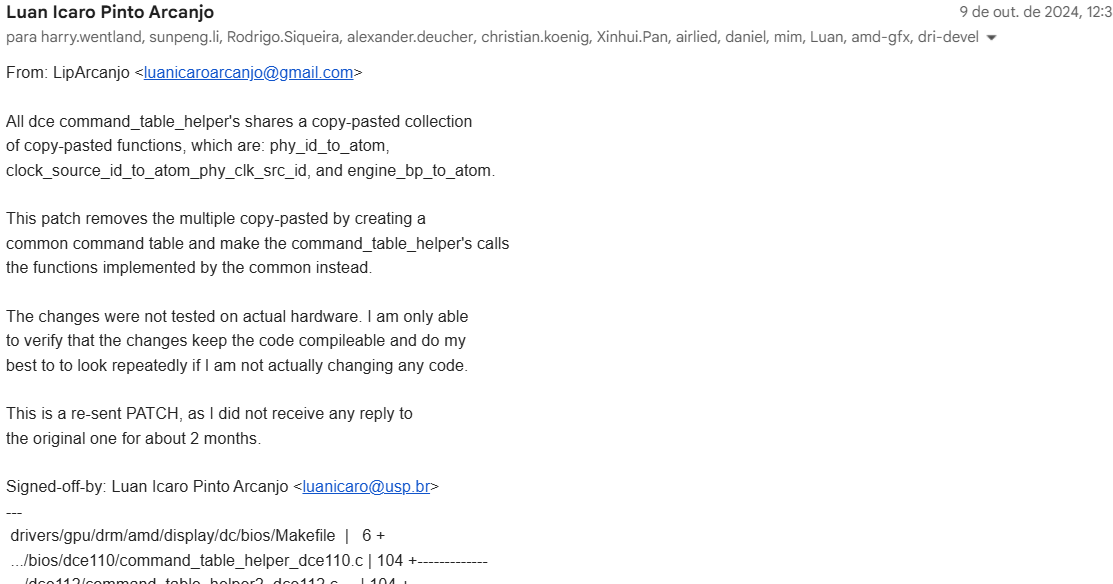
\includegraphics[scale=0.63]{patch_header}
\caption{Patch header for the second time send}
\label{fig:patch_header}
\end{figure}

\section{Patch initial reply}

\begin{figure}
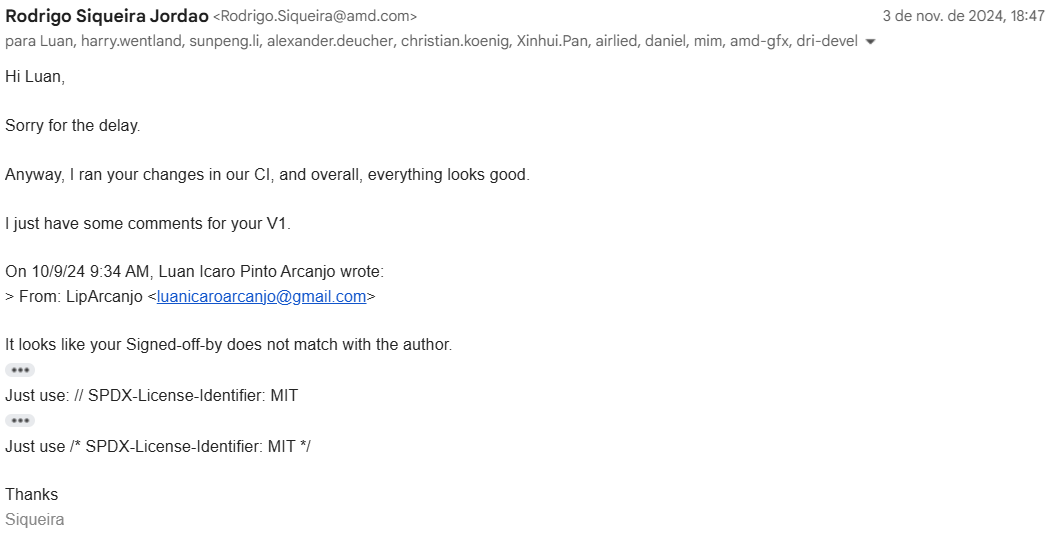
\includegraphics[scale=0.63]{patch_reply}
\caption{Patch initial reply message}
\label{fig:patch_reply}
\end{figure}

\par



%%%% Anexos %%%%

\cleardoublepage

%\pagestyle{appendix} % repete o anterior, caso você não use apêndices

%\annex

% \addappheadtotoc acrescenta a palavra "Anexo" ao sumário; se
% só há anexos, sem apêndices, provavelmente não é necessário.
%\addappheadtotoc

%%!TeX root=../tese.tex
%("dica" para o editor de texto: este arquivo é parte de um documento maior)
% para saber mais: https://tex.stackexchange.com/q/78101

\chapter{As packages \pkg{imegoodies} e \pkg{imelooks}}
\label{ann:imegoodlooks}

Este modelo inclui as \textit{packages} \pkg{imegoodies} e \pkg{imelooks},
que você pode querer usar em outros documentos \LaTeX.

\pkg{imegoodies} inclui um grande número de \textit{packages} que são
comumente usadas e bastante úteis. Em geral, você pode incluí-la em seus
documentos sem que isso cause problemas de compatibilidade. Se, no
entanto, algo não funcionar, você pode editar o arquivo para eliminar
a \textit{package} responsável pelo problema se ela não for necessária.
\pkg{imegoodies} ainda inclui vários comentários explicativos sobre as
\textit{packages} carregadas.

\pkg{imelooks} também inclui um grande número de \textit{packages}, mas
estas são relacionadas mais explicitamente à aparência do documento
(fontes, cores, margens etc.). Você também pode utilizá-la em outros
documentos se quiser se aproximar da aparência deste modelo. \pkg{imelooks}
reconhece diversos parâmetros que ativam/desativam aspectos específicos:

\begin{itemize}
  \item \cmd{fonts} carrega as fontes deste modelo (libertinus e
        sourcecodepro), além de outros pequenos ajustes relacionados.
        Esta opção é sempre ativada por padrão; para desativá-la, use
        \cmd{nofonts}

  \item \cmd{spacing} utiliza os espaçamentos definidos neste modelo (margens,
        espaço entre parágrafos, indentação da primeira linha do parágrafo
        etc.). Esta opção é sempre ativada por padrão; para desativá-la, use
        \cmd{nospacing}

  \item \cmd{captions} e \cmd{footnotes} fazem respectivamente as legendas
        (das figuras e tabelas) e as notas de rodapé de acordo com este modelo.
        Estas opções são sempre ativadas por padrão; para desativá-las, use
        \cmd{nocaptions} e \cmd{nofootnotes}

  \item \cmd{autohttp} acrescenta o prefixo \cmd{http://} a URLs criadas
        com \ltxcmd{url} que não incluam o \textit{schema}. Esta opção é
        sempre ativada por padrão; para desativá-la, use \cmd{noautohttp}

  \item \cmd{hidelinks}, \cmd{borderlinks} e \cmd{colorlinks} definem a
        aparência dos hiperlinks. \cmd{hidelinks} faz os hiperlinks sem
        nenhuma formatação especial; \cmd{borderlinks} faz os hiperlinks
        serem envidos por um quadrado colorido (apenas na tela; o quadrado
        não é impresso); \cmd{colorlinks} faz o texto dos hiperlinks ser
        colorido. A opção \cmd{colorlinks} é sempre ativada por padrão

  \item \cmd{biblatex} carrega a \textit{package} \cmd{biblatex} e os
        estilos bibliográficos deste modelo. Esta opção é sempre ativada
        por padrão; para desativá-la, use \cmd{nobiblatex}
  \item \cmd{raggedbib} faz a bibliografia (com \cmd{biblatex}) ser
        formatada com alinhamento à esquerda ao invés de justificado.
        Esta opção é sempre ativada por padrão, exceto quando o estilo
        bibliográfico é \cmd{plainnat-ime} (usado nas teses); para
        desativá-la, use \cmd{noraggedbib}; para ativá-la incondicionalmente,
        use \cmd{raggedbib}
  \item \cmd{bibstyle=?} selectiona um estilo bibliográfico específico.
        O estilo padrão é \cmd{numeric}, exceto em pôsteres e apresentações
        (\cmd{beamer-ime}) e \textit{reports} (\cmd{plainnat-ime})

  \item \cmd{listings} carrega a \textit{package} \cmd{listings} e diversas
        configurações relacionadas usadas neste modelo. Esta opção é
        sempre ativada por padrão; para desativá-la, use \cmd{nolistings}

  \item \cmd{greeny}, \cmd{bluey}, \cmd{sandy} ativam esquemas de cores
        diferentes para pôsteres e apresentações (o padrão é \cmd{bluey})

  \item \cmd{beamer} \textbf{des}ativa algumas \textit{packages} que
        são incompatíveis com a classe \cmd{beamer} (note que as opções
        \cmd{slides} e \cmd{presentation}, discutidas abaixo, já fazem isso)

  \item \cmd{presentation} (ou \cmd{slides}) e \cmd{poster} ativam as
        opções relevantes para, respectivamente, apresentações com
        \cmd{beamer} ou pôsteres com \cmd{tcolorbox}

  \item \cmd{report} ativa as opções relevantes para documentos com
        capítulos (cabeçalhos das páginas, características do sumário etc.)

  \item \cmd{thesis} ativa a opção \cmd{report} e também define o que é
        necessário para a geração da capa das teses de acordo com este modelo

  \item \cmd{resumoabstract} define os comandos \cmd{resumo} e \cmd{abstract}
        de acordo com este modelo. Esta opção é ativada por padrão com
        \cmd{report}; para desativá-la, use \cmd{noresumoabstract}

  \item \cmd{brazilian} verifica se a língua portuguesa está ativa no
        documento e, em caso negativo, gera um erro. Esta opção é
        ativada por padrão com a opção \cmd{thesis}; para desativá-la,
        use \cmd{nobrazilian}
\end{itemize}

%\par
%%!TeX root=../tese.tex
%("dica" para o editor de texto: este arquivo é parte de um documento maior)
% para saber mais: https://tex.stackexchange.com/q/78101

\chapter{Código-fonte e pseudocódigo}
\label{ap:pseudocode}

Com a \textit{package} \textsf{listings}, programas podem ser inseridos
diretamente no arquivo, como feito no caso do Programa~\ref{prog:java},
ou importados de um arquivo externo com o comando
\textsf{\textbackslash{}lstinputlisting}, como no caso
do Programa~\ref{prog:mdcinput}.

% O exemplo foi copiado da documentação de algorithmicx
\begin{program}
  \lstinputlisting[
    language=pseudocode,
    style=pseudocode,
    style=wider,
    functions={},
    specialidentifiers={},
  ]
  {conteudo/euclid.psc}

  \caption{Máximo divisor comum (arquivo importado).\label{prog:mdcinput}}
\end{program}

Trechos de código curtos (menores que uma página) podem ou não ser
incluídos como \textit{floats}; trechos longos necessariamente incluem
quebras de página e, portanto, não podem ser \textit{floats}. Com
\textit{floats}, a legenda e as linhas separadoras são colocadas pelo
comando \textsf{\textbackslash{}begin\{program\}}; sem eles, utilize o
ambiente \textsf{programruledcaption} (atenção para a colocação do
comando \textsf{\textbackslash{}label\{\}}, dentro da legenda), como
no Programa~\ref{prog:mdc}\footnote{\textsf{listings} oferece alguns
recursos próprios para a definição de \textit{floats} e legendas, mas
neste modelo não os utilizamos.}:

\begin{programruledcaption}{Máximo divisor comum (em português).\label{prog:mdc}}
  \begin{lstlisting}[
    language={[brazilian]pseudocode},
    style=pseudocode,
    style=wider,
    functions={},
    specialidentifiers={},
  ]
      funcao euclides(a, b) // O máximo divisor comum de \textbf{a} e \textbf{b}
          r := a $\bmod$ b
	  enquanto r != 0 // Atingimos a resposta se \textbf{r} é zero
              a := b
              b := r
              r := a $\bmod$ b
          fim
	  devolva b // O máximo divisor comum é \textbf{b}
      fim
  \end{lstlisting}
\end{programruledcaption}

Além do suporte às várias linguagens incluídas em \textsf{listings},
este modelo traz uma extensão para permitir o uso de pseudocódigo,
útil para a descrição de algoritmos em alto nível. Ela oferece
diversos recursos:

\begin{itemize}

    \item Comentários seguem o padrão de C++ (\lstinline{//} e
          \lstinline{/* ... */}), mas o delimitador é impresso
          como ``$\triangleright$''.

    \item ``:='', ``<>'', ``<='', ``>='' e ``!='' são substituídos
          pelo símbolo matemático adequado.

    \item É possível acrescentar palavras-chave além de ``if'', ``and''
          etc. com a opção ``\textsf{morekeywords=\{pchave1,\linebreak[0]{}pchave2\}}''
          (para um trecho de código específico) ou com o comando
          \textsf{\textbackslash{}lstset\{morekeywords=\linebreak[0]{}\{pchave1,pchave2\}\}}
          (como comando de configuração geral).

    \item É possível usar pequenos trechos de código, como nomes de variáveis,
          dentro de um parágrafo normal com \textsf{\textbackslash{}lstinline\{blah\}}.

    \item ``\$\dots\$'' ativa o modo matemático em qualquer lugar.

    \item Outros comandos \LaTeX{} funcionam apenas em comentários; fora, a
          linguagem simula alguns pré-definidos (\textsf{\textbackslash{}textit\{\}},
          \textsf{\textbackslash{}texttt\{\}} etc.).

    \item O comando \textsf{\textbackslash{}label} também funciona em
          comentários; a referência correspondente (\textsf{\textbackslash{}ref})
          indica o número da linha de código. Se quiser usá-lo numa linha sem
          comentários, use \lstinline{///}~\textsf{\textbackslash{}label\{blah\}};
          ``\lstinline{///}'' funciona como \lstinline{//}, permitindo
          a inserção de comandos \LaTeX{}, mas não imprime o delimitador
          (\ensuremath{\triangleright}).

    \item Para suspender a formatação automática, use \textsf{\textbackslash{}noparse\{blah\}}.

    \item Para forçar a formatação de um texto como função, identificador,
          palavra-chave ou comentário, use \textsf{\textbackslash{}func\{blah\}},
          \textsf{\textbackslash{}id\{blah\}}, \textsf{\textbackslash{}kw\{blah\}} ou
          \textsf{\textbackslash{}comment\{blah\}}.

    \item Palavras-chave dentro de comentários não são formatadas
          automaticamente; se necessário, use \textsf{\textbackslash{}func\{\}},
          \textsf{\textbackslash{}id\{\}} etc. ou comandos \LaTeX{} padrão.

    \item As palavras ``Program'', ``Procedure'' e ``Function'' têm formatação
          especial e fazem a palavra seguinte ser formatada como função.
          Funções em outros lugares \emph{não} são detectadas automaticamente;
          use \textsf{\textbackslash{}func\{\}}, a opção ``\textsf{functions=\{func1,func2\}}''
          ou o comando ``\textsf{\textbackslash{}lstset\{functions=\{func1,func2\}\}}''
          para que elas sejam detectadas.

    \item Além de funções, palavras-chave, strings, comentários e
          identificadores, há ``\textsf{specialidentifiers}''. Você pode
          usá-los com \textsf{\textbackslash{}specialid\{blah\}}, com a opção
          ``\textsf{specialidentifiers=\{id1,id2\}}'' ou com o comando
          ``\textsf{\textbackslash{}lstset\{specialidentifiers=\{id1,id2\}\}}''.

\end{itemize}



%\par


%%%%%%%%%%%%%%% SEÇÕES FINAIS (BIBLIOGRAFIA E ÍNDICE REMISSIVO) %%%%%%%%%%%%%%%%

% O comando backmatter desabilita a numeração de capítulos.
\backmatter

\pagestyle{backmatter}

% Espaço adicional no sumário antes das referências / índice remissivo
\addtocontents{toc}{\vspace{2\baselineskip plus .5\baselineskip minus .5\baselineskip}}

% A bibliografia é obrigatória

\printbibliography[
  title=\refname\label{sec:bib}, % "Referências", recomendado pela ABNT
  %title=\bibname\label{sec:bib}, % "Bibliografia"
  heading=bibintoc, % Inclui a bibliografia no sumário
]

%\printindex % imprime o índice remissivo no documento (opcional)

\end{document}
